% CHAPTER 4
\chapter[Nucleic Acid Systems]{Electronic Structure for Nucleic Acid Systems}

Having established the foundations of quantum chemistry for condensed
matter systems, we now turn our attention to nucleic acids.  Modern
molecular biology has focused a great deal of attention toward
understanding the structure and function of this class of molecule.
The very first quantum chemical calculations on DNA\cite{LADIK1964} by
Ladik and Hoffman date back to 1964 and were focused primarily on
semiempirical treatments of the band structure.



\section{Start Small:  Early Studies of DNA Bases}
An impressive body of work concerning small numbers of DNA bases has
come from the collaboration of Ji\u{r}\'{i} \v{S}poner, Pavel Hobza,
and Jerzy
Leszczynski.\cite{Sponer1994,Sponer2001a,Sponer02,Reha02,Sponer04,Sponer2005a,Perez2005,Kabelac2007}

Our examination of larger systems relies on the fundamental
description of the electronic structure of smaller

\begin{figure}[tb]
  \newlength{\panelwidth}
  \setlength{\panelwidth}{0.485\textwidth}
  \newlength{\capwidth}
  \setlength{\capwidth}{\textwidth}
  \begin{tabular}{lr}
    \begin{minipage}{\panelwidth}
      \includegraphics[width=\panelwidth]{YP-01.cations.B3LYP-STO3G.ecce.DOS.eps}
    \end{minipage} &
    \begin{minipage}{\panelwidth}
      \includegraphics[width=\panelwidth]{YP-01.cations.B3LYP-SBK.ecce.DOS.eps}
    \end{minipage} \\
    \begin{minipage}{\panelwidth}\centering STO-3G\end{minipage} &
    \begin{minipage}{\panelwidth}\centering SBKJC ECP\end{minipage}\\[4ex]
    \multicolumn{2}{c}{
    \begin{minipage}{\capwidth}
        \caption{Comparison of the density of states plots for the
        sequence CGTAAGGGTTACA generated using the B3LYP density
        functional.
        \label{Fig:DOS_Comparison}}
    \end{minipage}} \\
  \end{tabular}
\end{figure}

Choice of basis set has a tremendous influence on the quality of the
results as illustrated by Figure \ref{Fig:DOS_Comparison}.
The two density of states\index{density of states} plots were
generated from the same d(CGTAAGGGTTACA) canonical double-helix with
counterions using the B3LYP density functional, with only the basis
set differing between the two calculations.  The most obvious
defference between these two calculations is the distribution of
states around the HOMO--LUMO gap. In the minimal basis calculation,
this gap is nearly 3 eV, whereas using the ECP basis set produces a
gap of less than 1 eV.  Furthermore, the energy of the HOMO in the
STO-3G calculation is positive, suggesting that the HOMO is an unbound
electron state.

A closer examination of the DOS plot for the B3LYP/SBKJC calculation
reveals some interesting and important features.  A collection of
states creates a peak between -2 and -1 eV just above the HOMO.  This
collection of empty states represents the unoccupied \textit{s}
orbitals on the Na counterions.  They are bound states and there is a
small gap between the HOMO of the oligonucleotide and the lower edge
of this unoccupied band.  Another important feature is the small
collection of unoccupied bound states just below 0 eV.  They are part
of a much larger set of states with a peak near 0.5 eV, but their
physical importance is tied to their negative energies.

As was discussed in the theoretical background, a semiconductor system
contains a set of unoccupied states with negative energy with the
Fermi gap separating the band of occupied and unoccupied states.  What
we see emerging in the calculations is the electronic structure of a
semiconductor system and the failure of the minimal basis set
treatment to describe this represents a serious shortcoming.  While
the ECP basis set neglects a direct treatment of the core orbitals, it
does describe the important features of the frontier molecular
orbitals with only a double-$\zeta$ quality basis set.

\begin{figure}[tb]
  % \newlength{\panelwidth}
  \setlength{\panelwidth}{0.485\textwidth}
  % \newlength{\capwidth}
  \setlength{\capwidth}{\textwidth}
  % \addtolength{\capwidth}{-6.0\tabcolsep}
  \begin{tabular}{lr}
    \begin{minipage}{\panelwidth}
      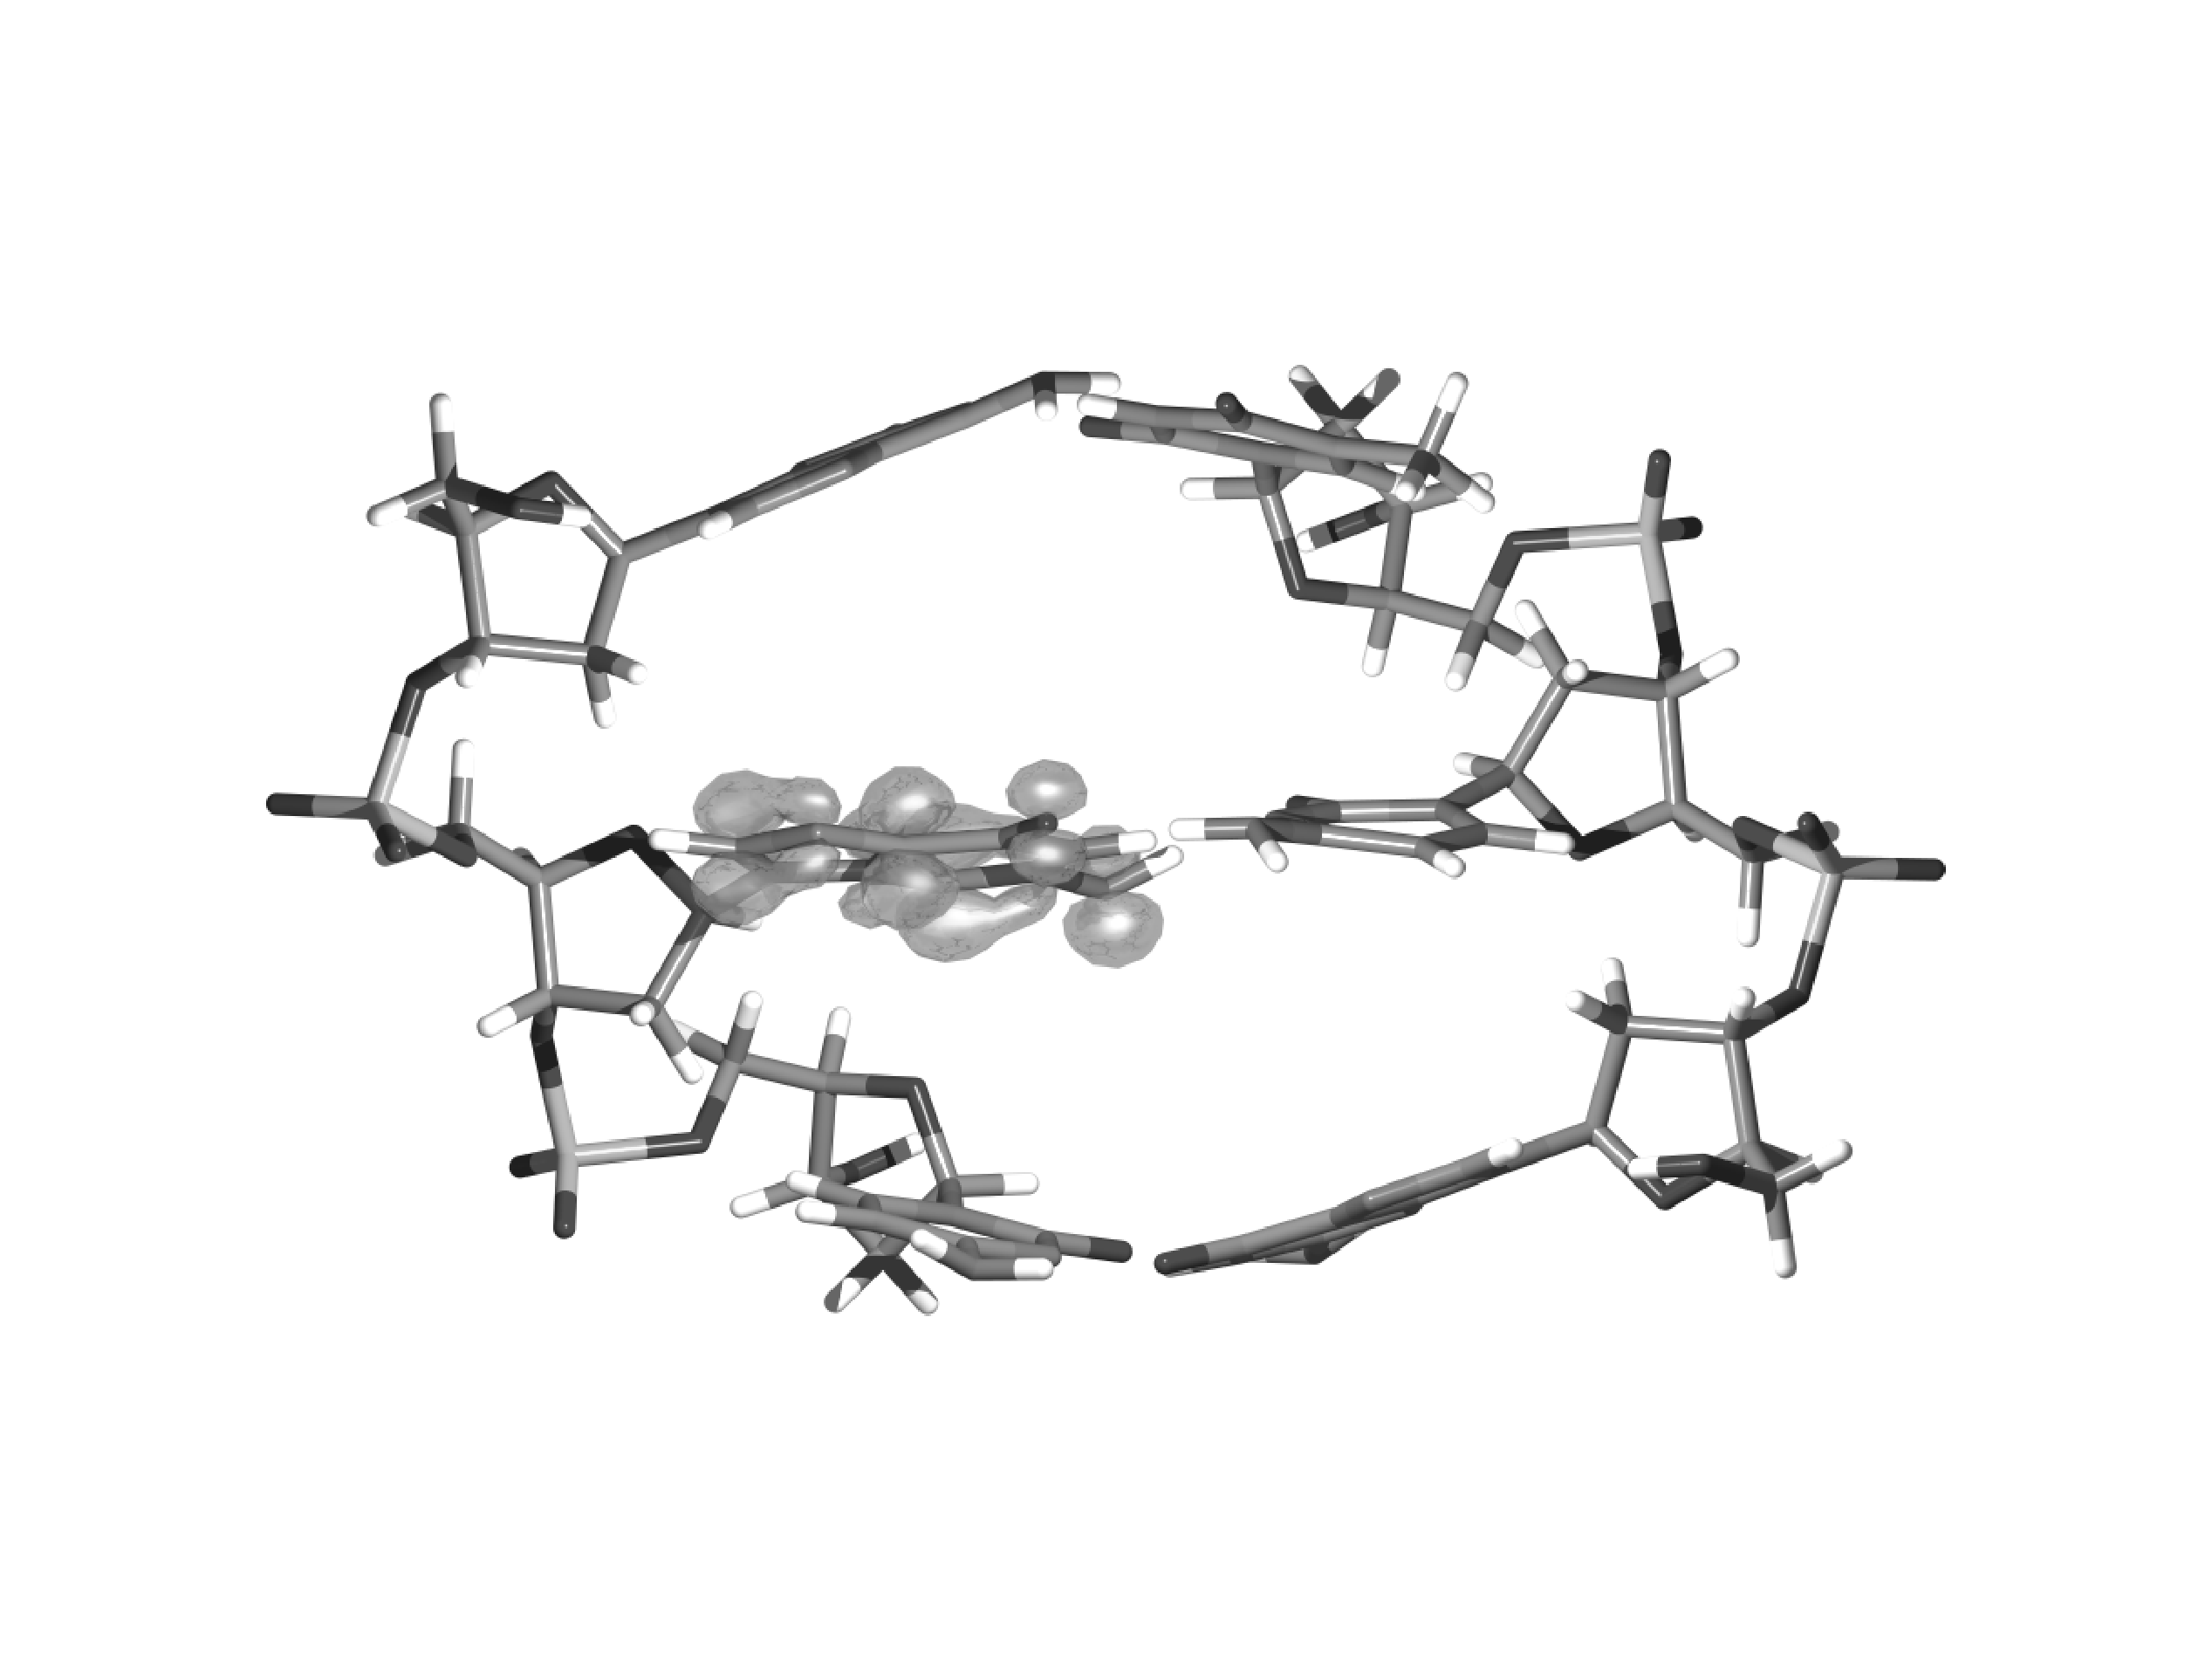
\includegraphics[width=\panelwidth]{DNA_Trimer_BasisSetDependence/AGC.B3LYP-321G.HOMO.eps}
    \end{minipage} &
    \begin{minipage}{\panelwidth}
      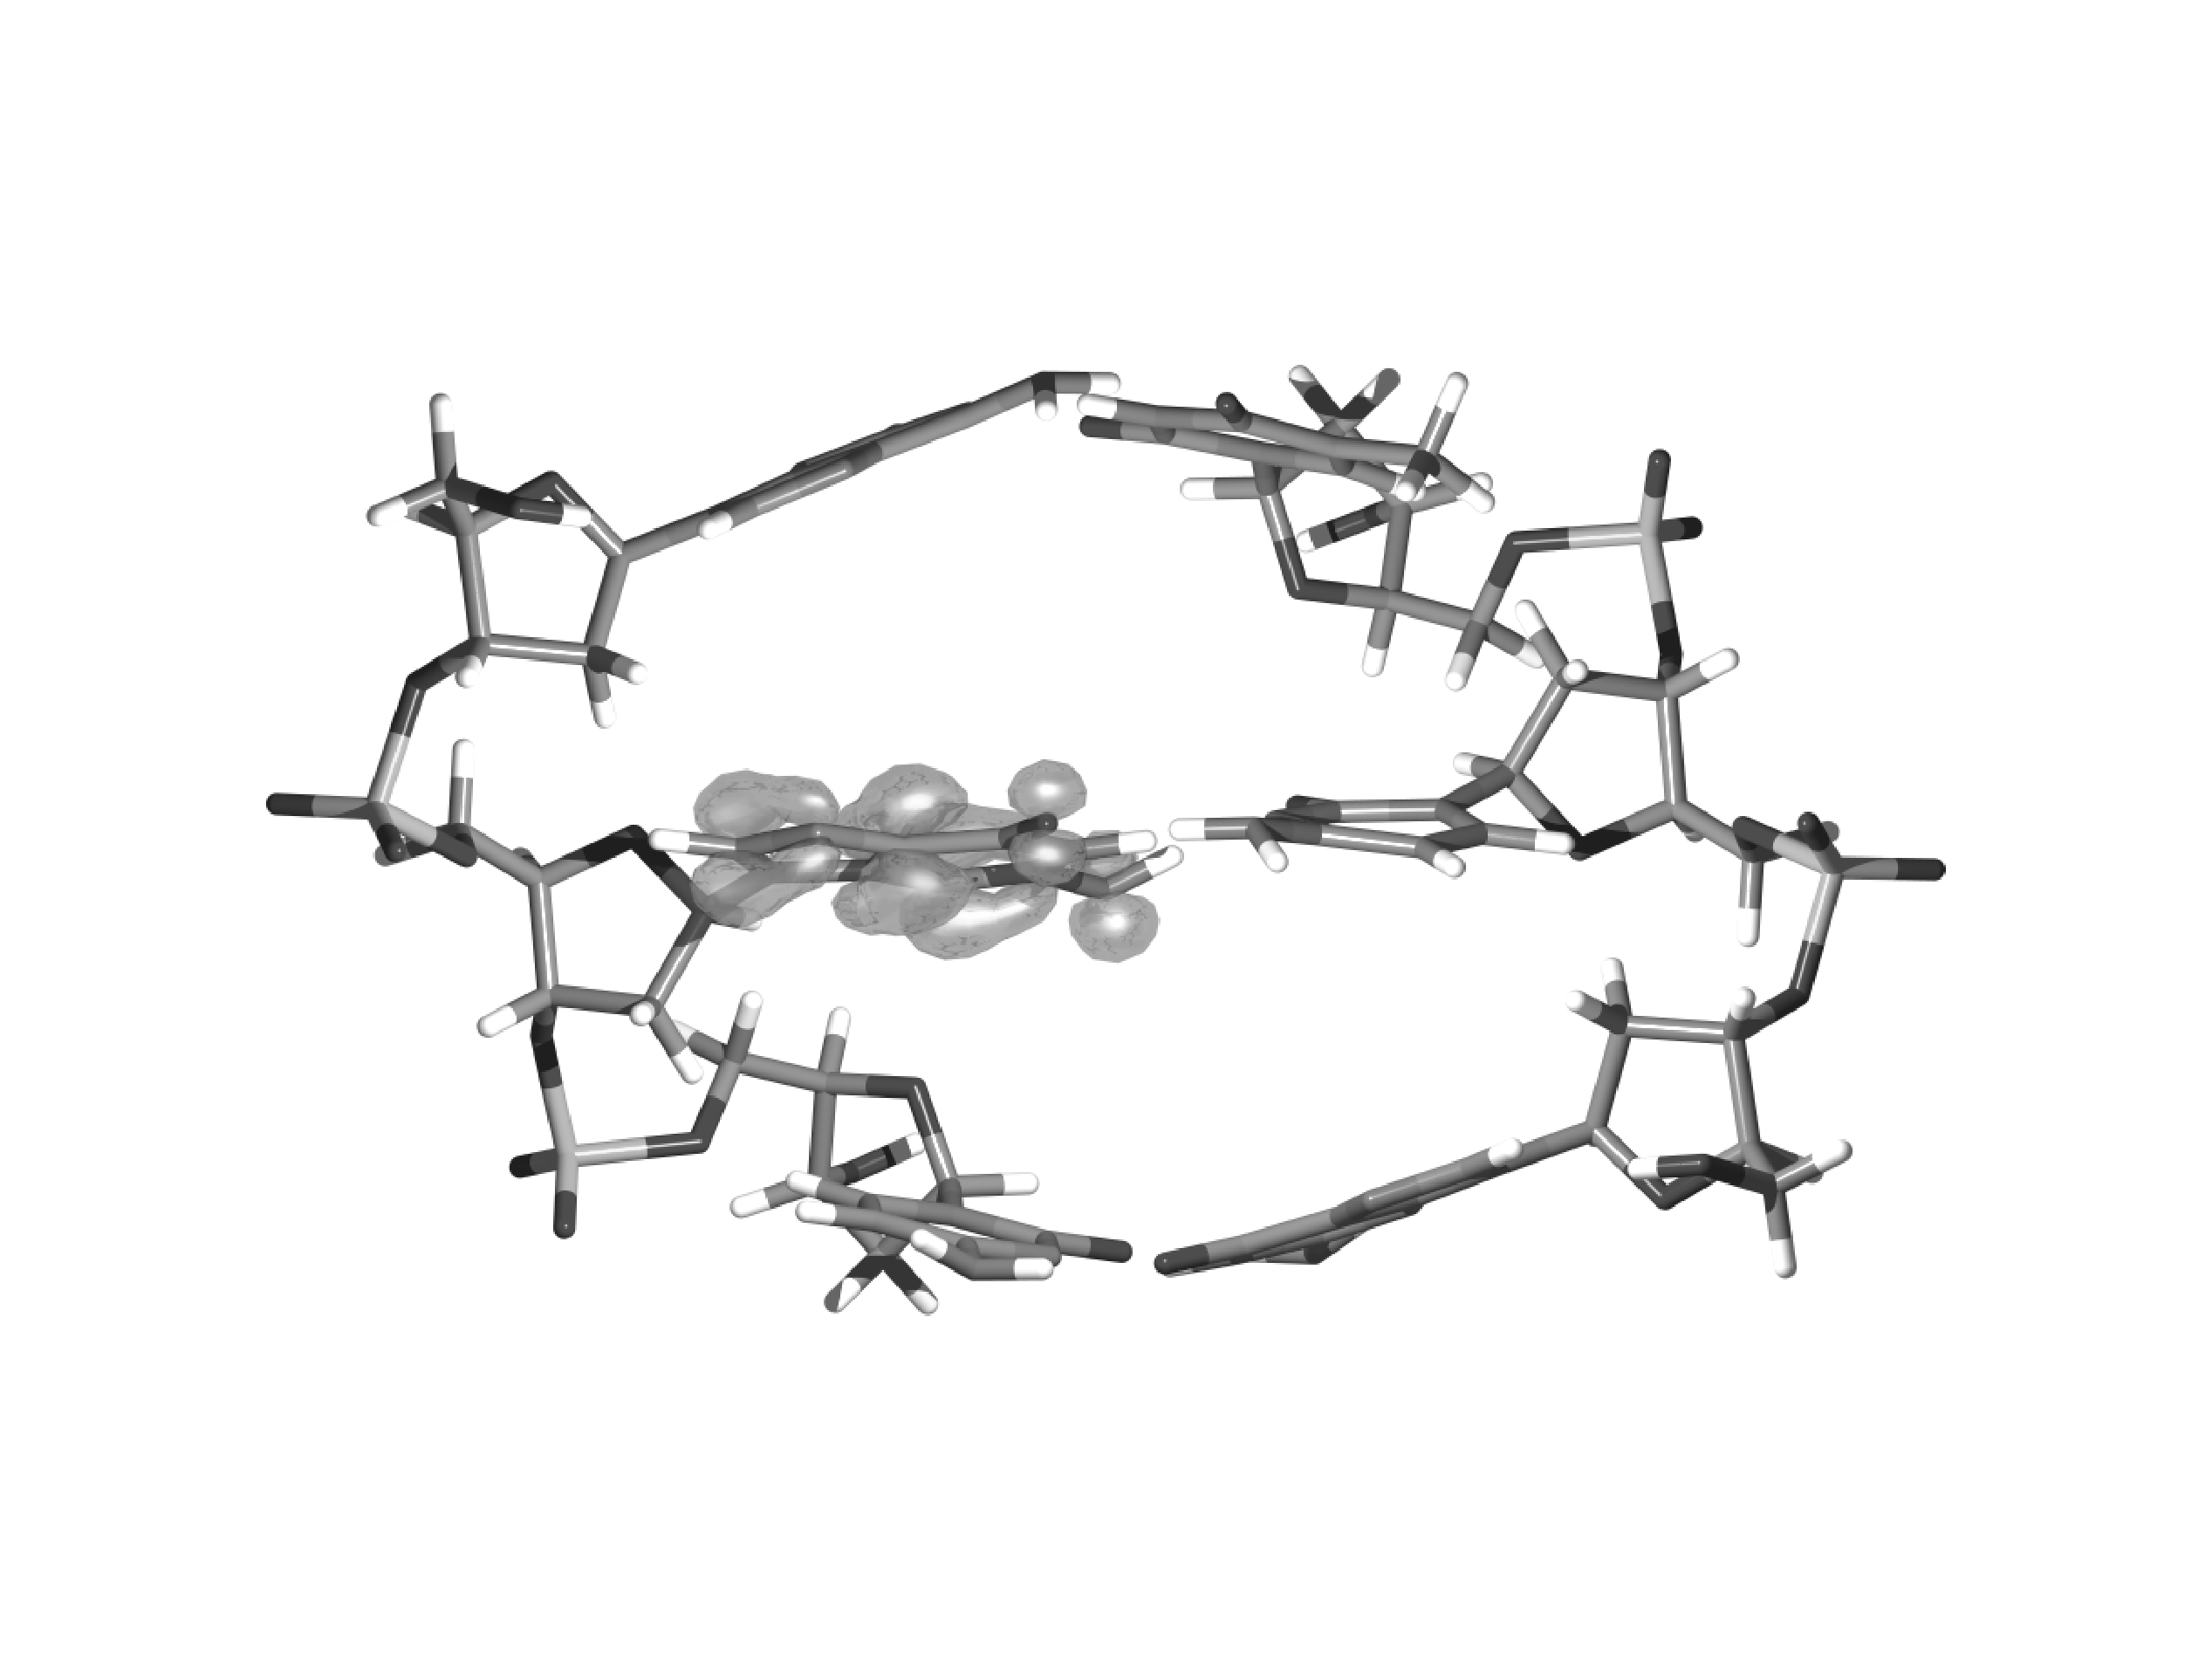
\includegraphics[width=\panelwidth]{DNA_Trimer_BasisSetDependence/AGC.B3LYP-ccpVTZ.HOMO.eps}
    \end{minipage} \\
    \begin{minipage}{\panelwidth}\centering 3-21G\end{minipage} &
    \begin{minipage}{\panelwidth}\centering cc-pVTZ\end{minipage}\\[4ex]
    \begin{minipage}{\panelwidth}
      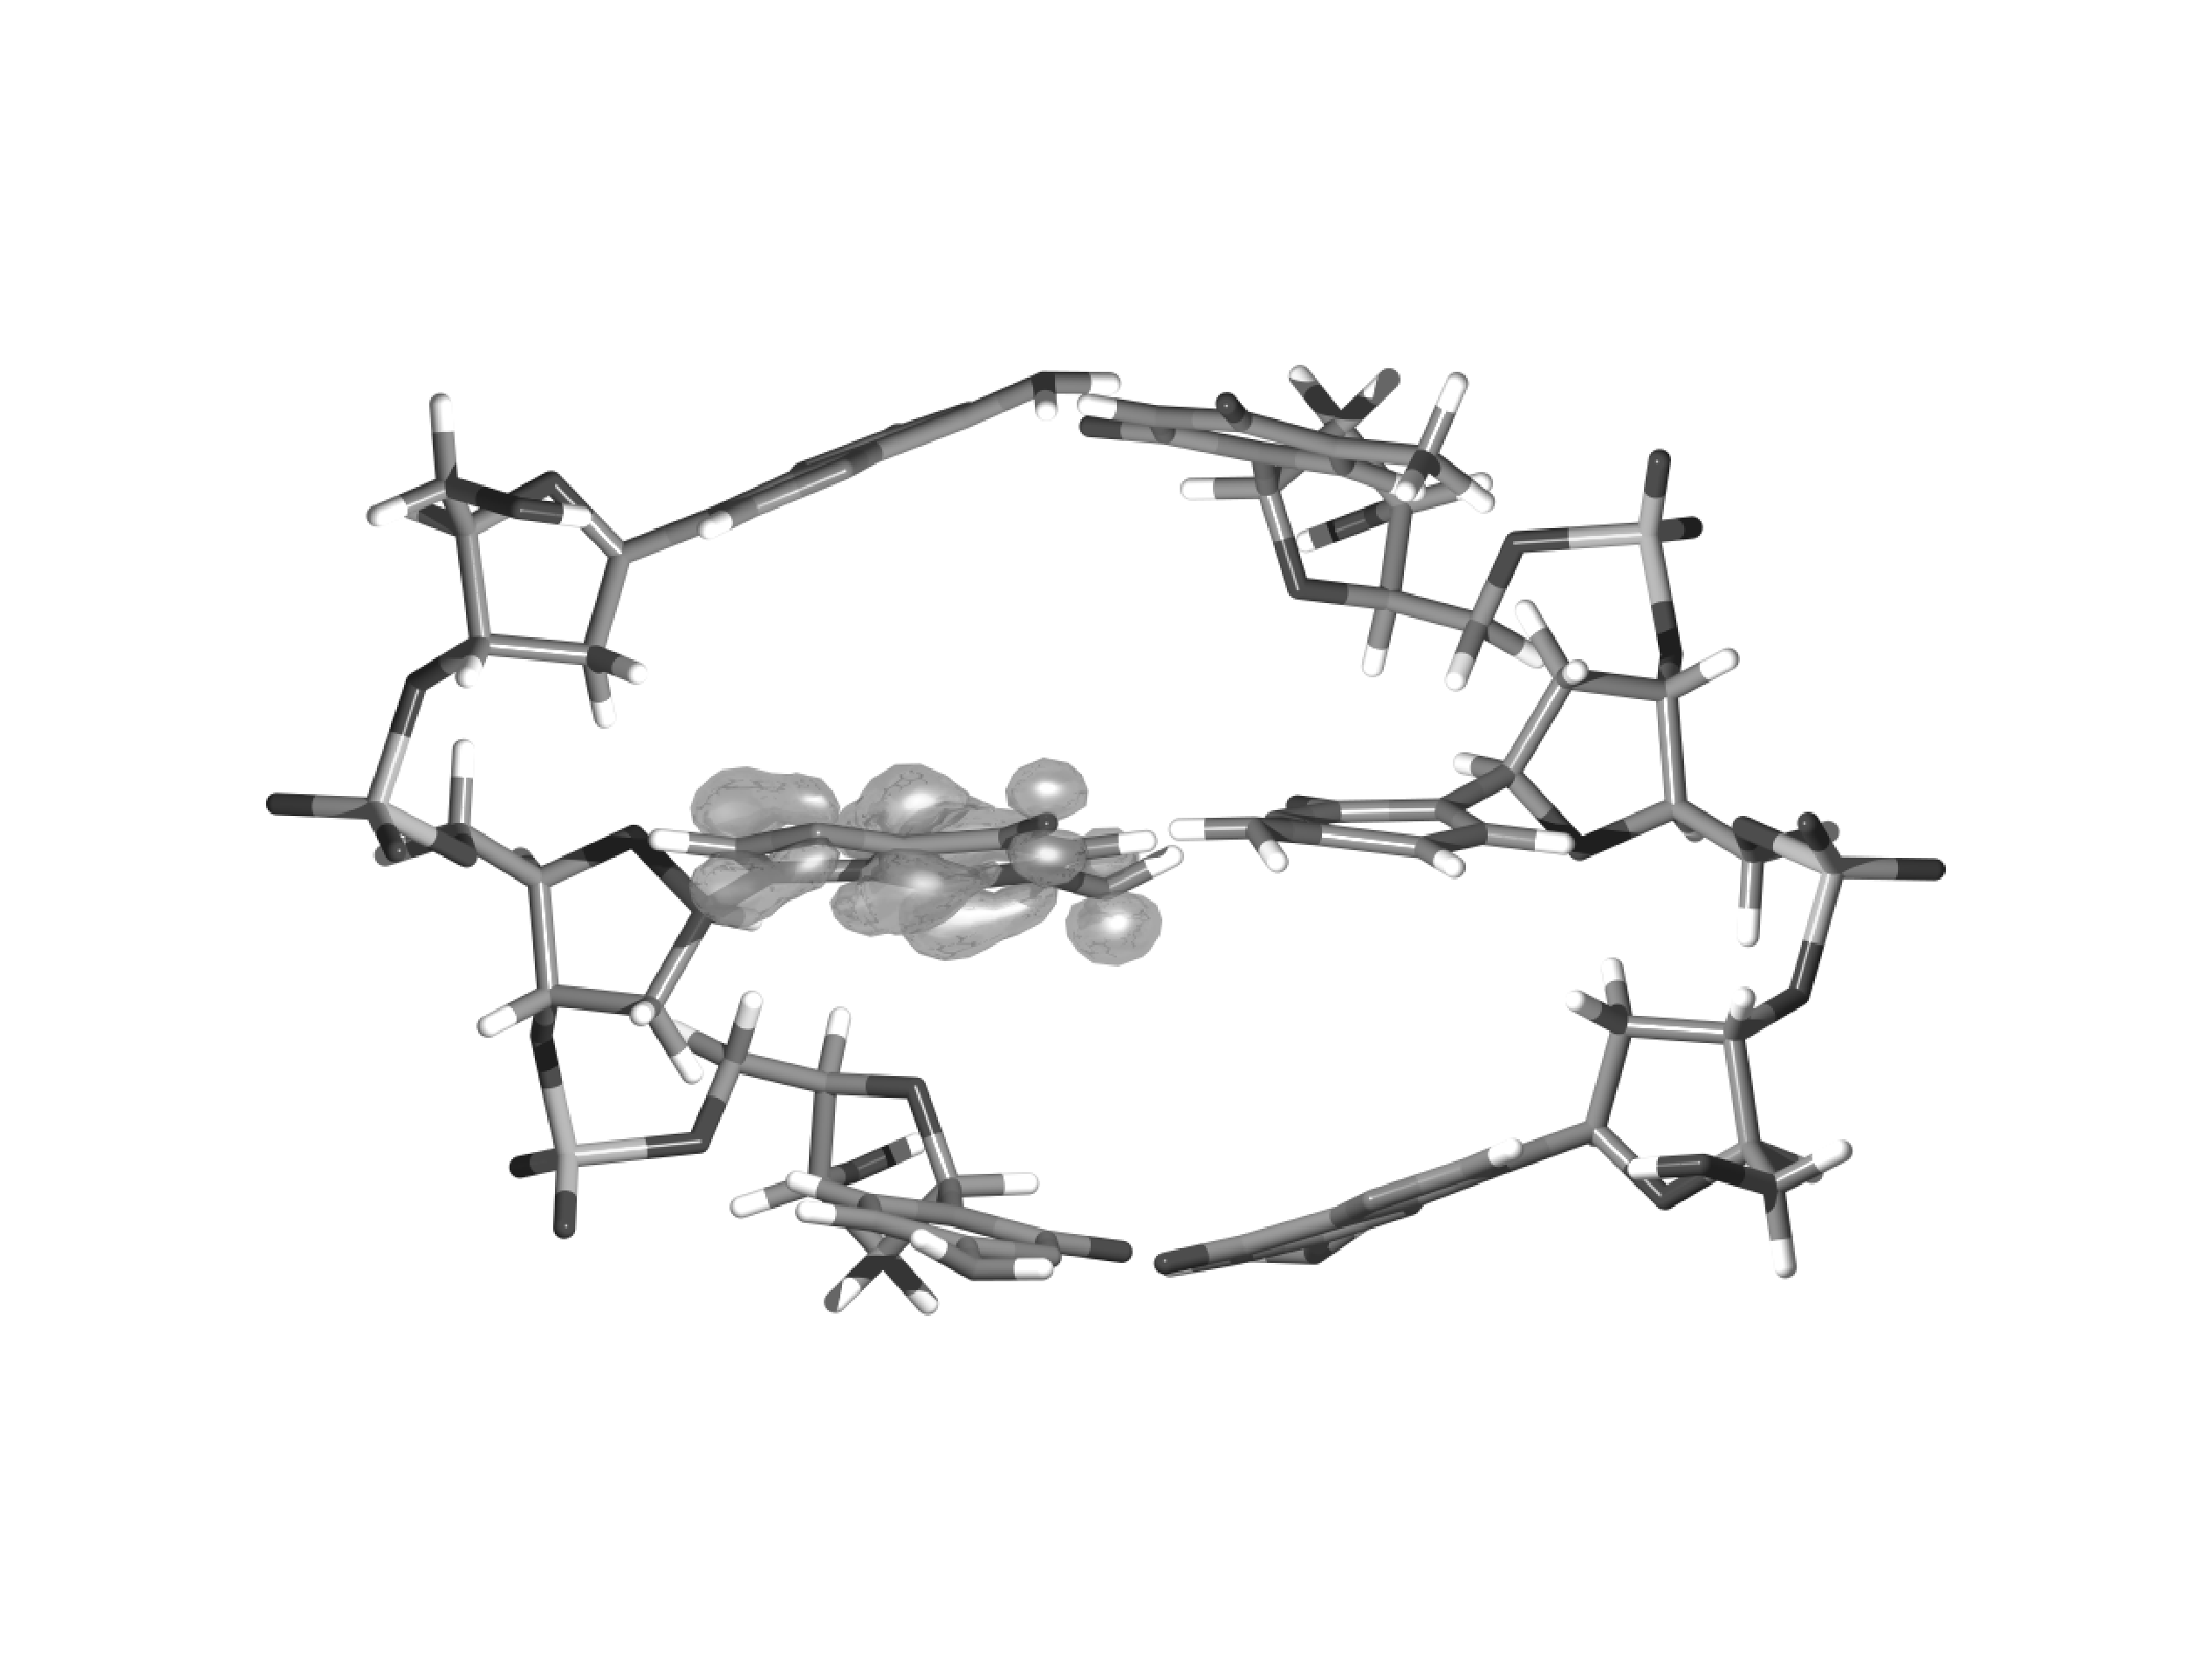
\includegraphics[width=\panelwidth]{DNA_Trimer_BasisSetDependence/AGC.B3LYP-pAhlrichs.HOMO.eps}
    \end{minipage} &
    \begin{minipage}{\panelwidth}
      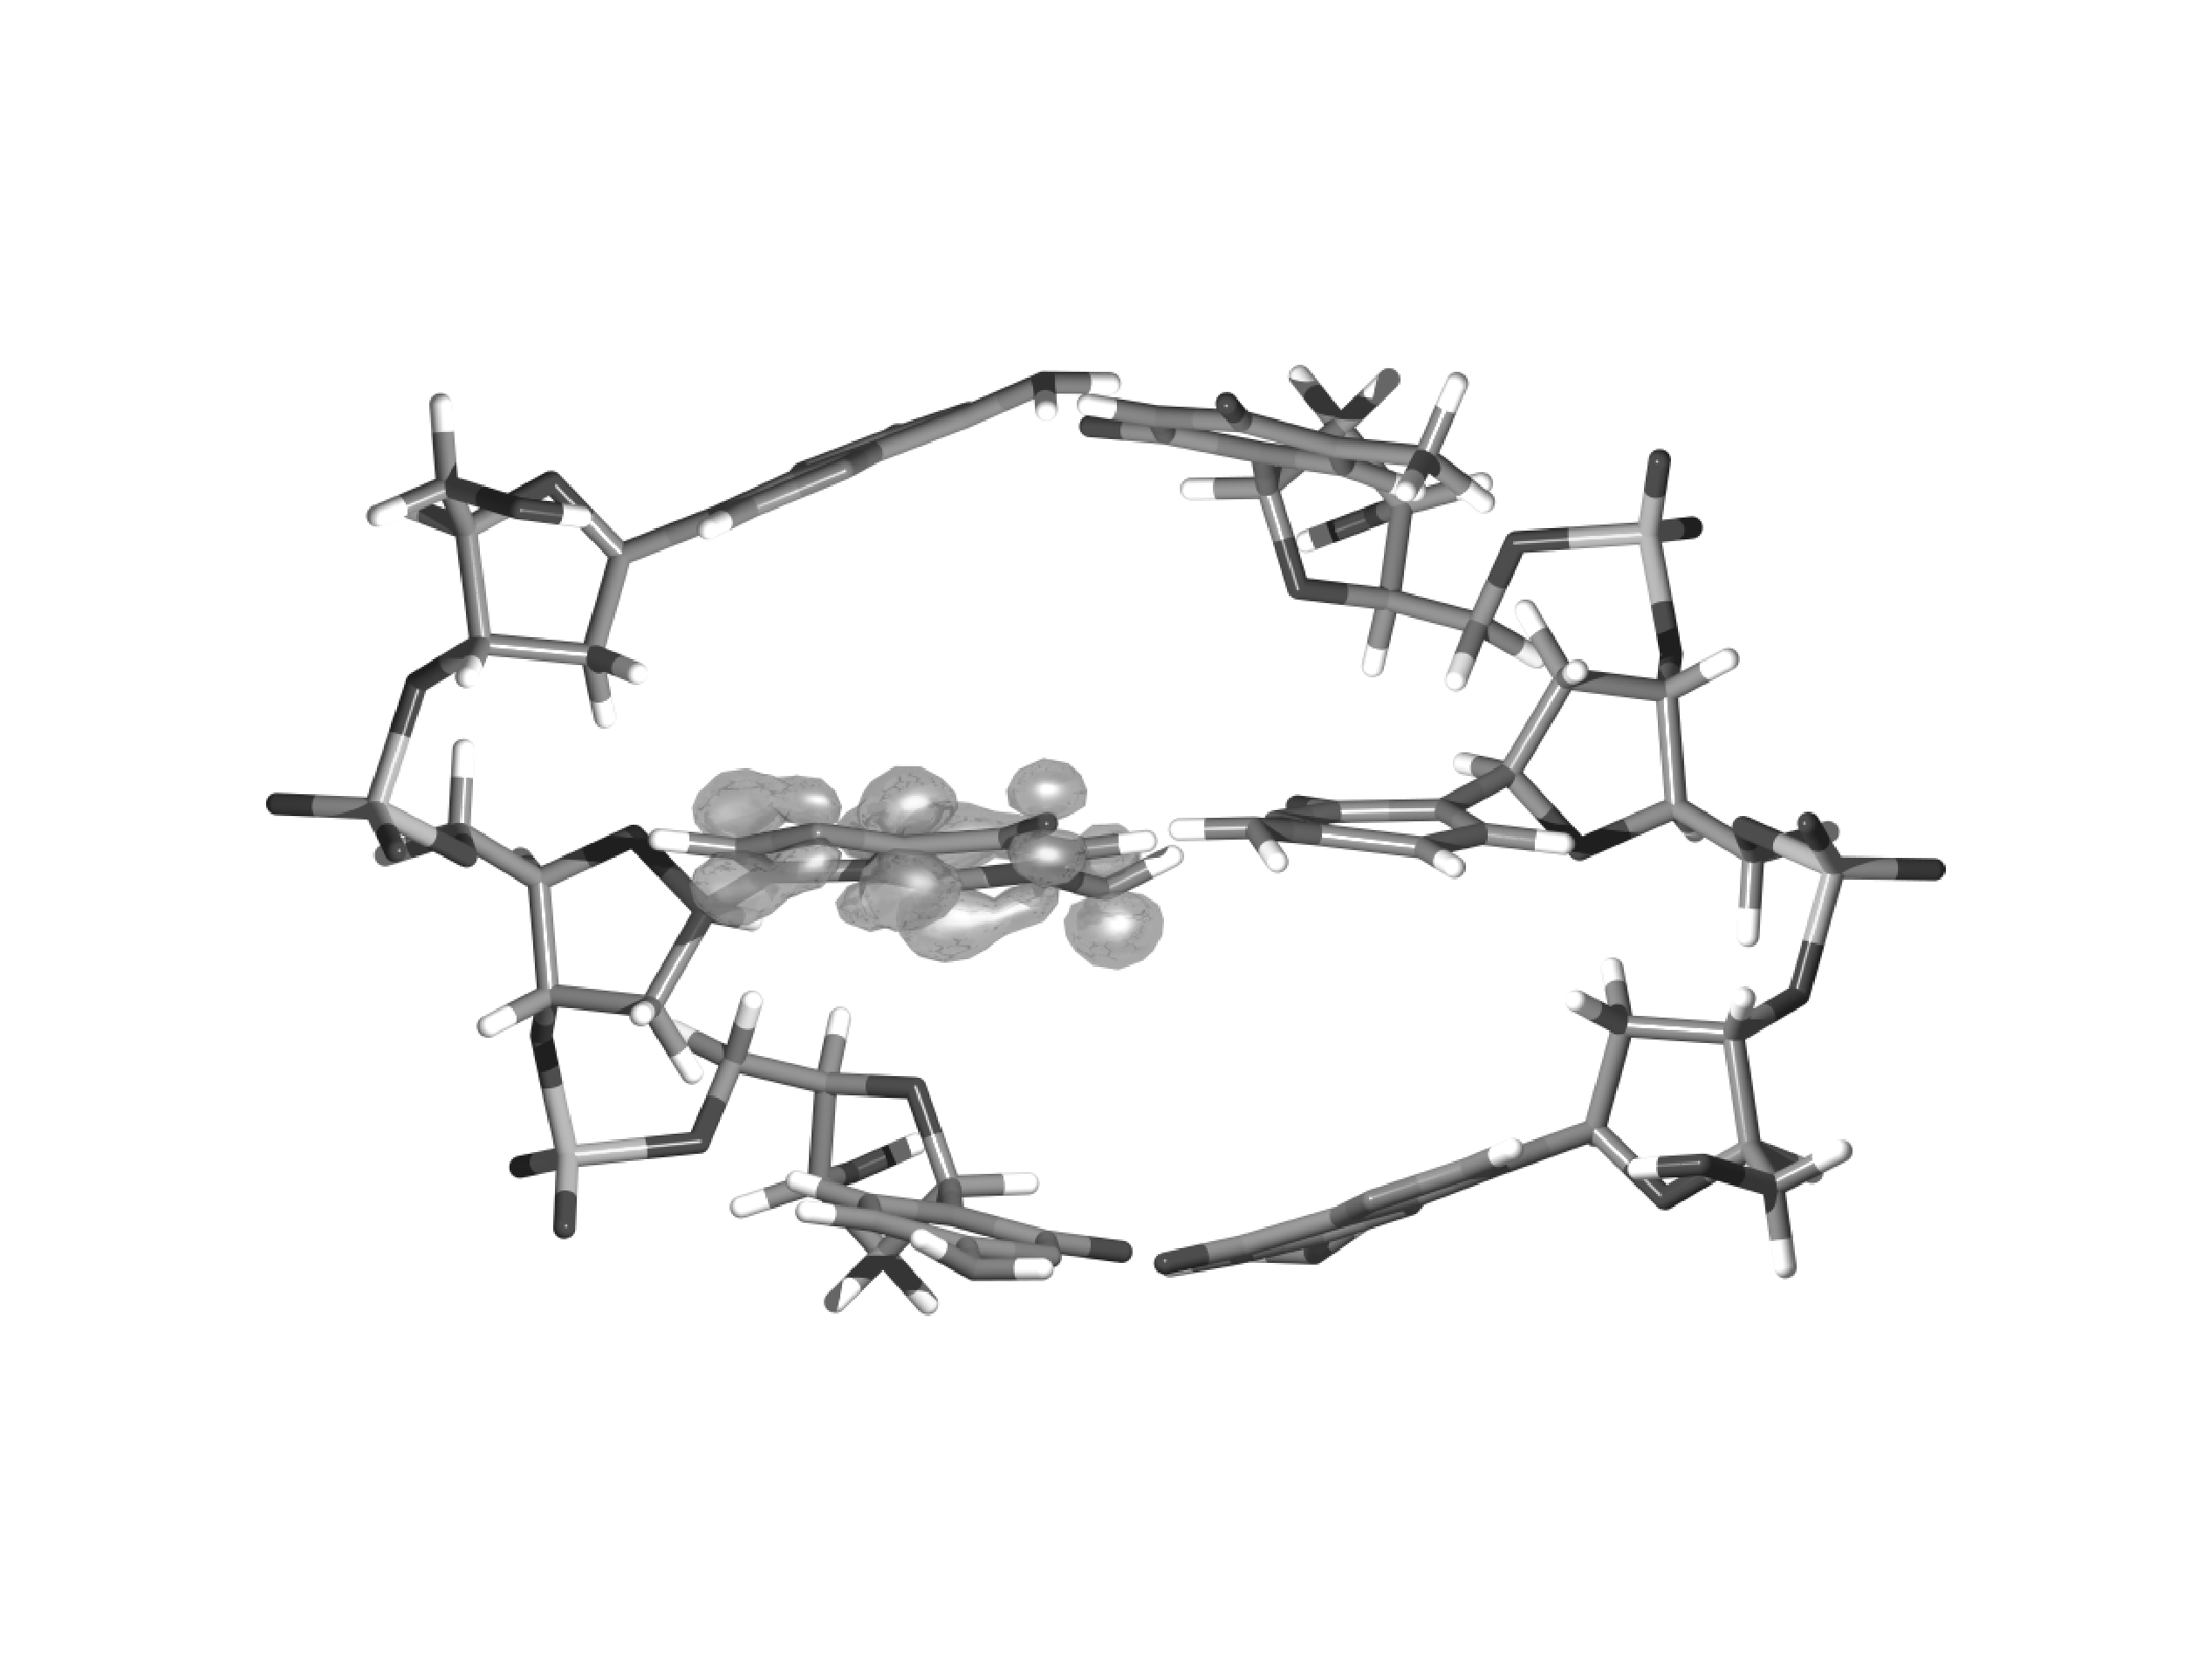
\includegraphics[width=\panelwidth]{DNA_Trimer_BasisSetDependence/AGC.B3LYP-SBK.HOMO.eps}
    \end{minipage} \\
    \begin{minipage}{\panelwidth}\centering p-Ahlrichs\end{minipage} &
    \begin{minipage}{\panelwidth}\centering SBKJC ECP\end{minipage}\\[4ex]
    \multicolumn{2}{c}{
    \begin{minipage}{\capwidth}
        \caption{Comparison of the highest occupied molecular orbital (HOMO)
        for the three base pair dsDNA (AGC) using four different AO basis sets.
        It is imporatnt to note that the qualitative description of the HOMO
        differs significantly for the 3-21G basis set versus the other three
        basis sets.  However, the double-$\zeta$ quality effective core
        potential gives a qualitative description nearly identical to that of
        the much higher-quality polarized basis sets.
        \label{Fig:HOMO_Comparison}}
    \end{minipage}} \\
  \end{tabular}
\end{figure}



\section{Large-scale Calculations of Electronic Structure}
Ultimately, the goal of any computational technique is to provide
insight into experiments that take place in the laboratory.
Biological system present an array of modelling challenges with scale
and complexity being foremost among them.  Molecules important to
biologists function in living systems and are therefore subject to an
extraordinarily complex network of interactions.  Properly describing
the environmental conditions in which these molecular species function
is often difficult, if not impossible.


\begin{figure}[tb]
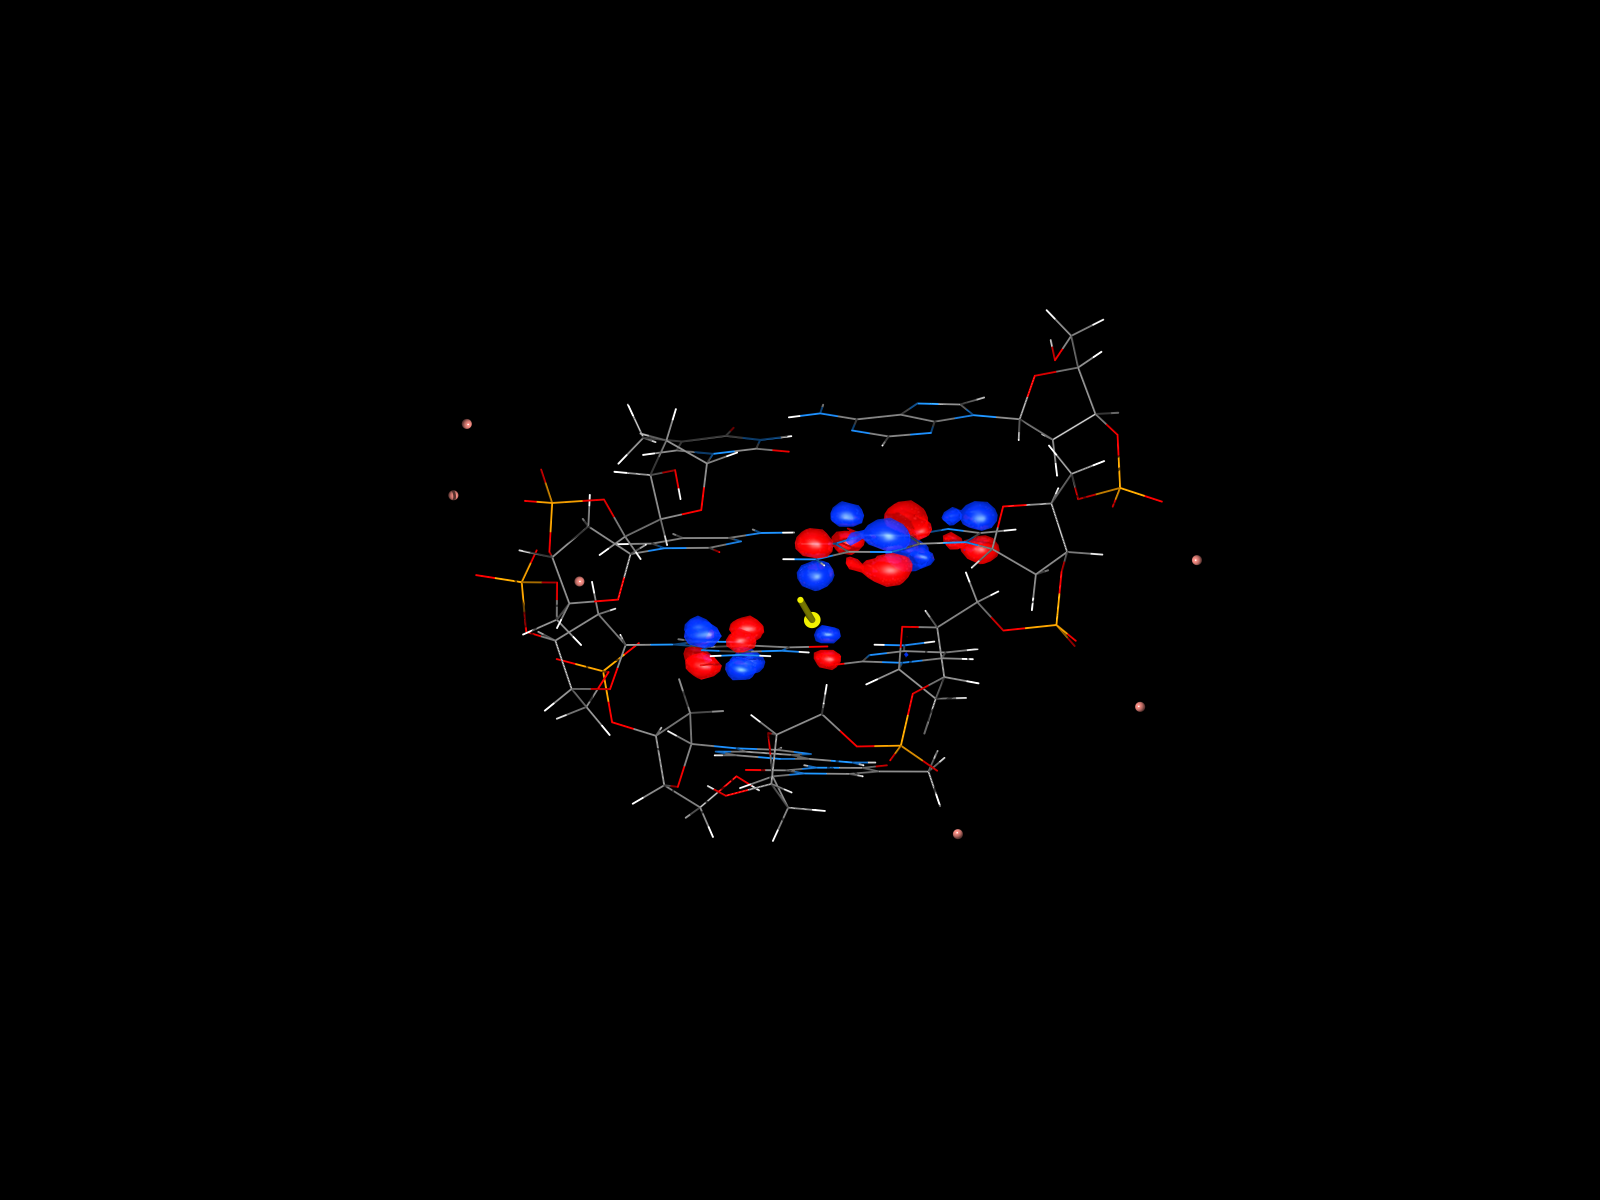
\includegraphics[width=\textwidth]{AGCT_SBK-HOMO.eps}
\caption{Orbital diagram for the HOMO of d(AGCT) obtained from B3LYP/SBKJC.\label{Fig:AGCT_HOMO}}
\end{figure}

\begin{figure}[tb]
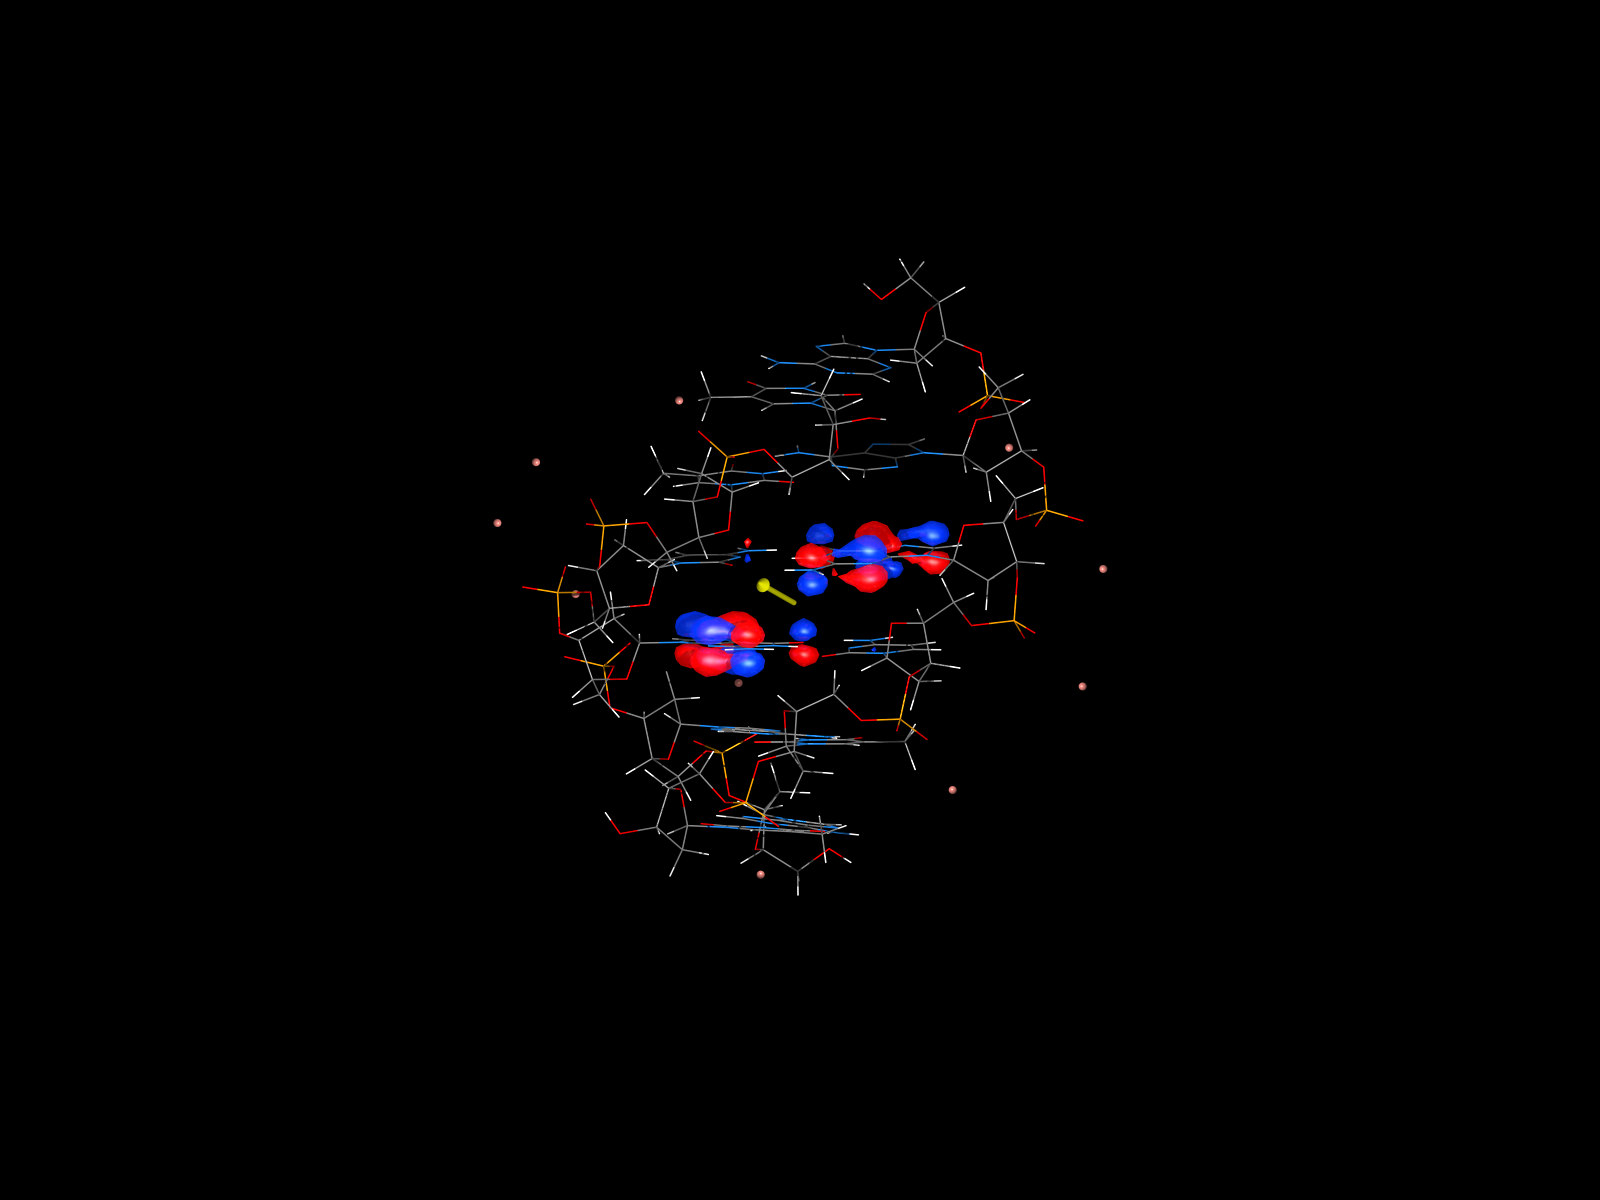
\includegraphics[width=\textwidth]{AAGCTT_SBK-HOMO.eps}
\caption{Orbital diagram for the HOMO of d(AAGCTT) obtained from B3LYP/SBKJC.\label{Fig:AAGCTT_HOMO}}
\end{figure}


\subsection{Convergence Issues}
Because nucleic acid systems carry significant negative charge in the
phosphate backbone, the treatment of increasing numbers of nucleobases
requires the solution of Hamiltonians associated with increasing
diffuse orbitals.

In practice, this means that systems containing more than eight base
pairs are impossible to converge to a stable wavefunction.
Convergence of the SCF procedure can be achieved for sequences of up
to eight base pairs by treating only the DNA atoms with an appropriate
total charge derived from the number of phosphate groups in the
backbone.  This is possible because the excess negative charge resides
in the phosphate oxygen atoms rather than throughout the molecule.
Unfortunately this phenomenon, which allows the treatment of
medium-sized systems, causes problems when going beyond eight base
pairs.  Mixing of the valence shell AOs on the exocyclic oxygen atoms
occurs with larger systems and hinders SCF convergence to the point of
failure, even when given very large (> 200) numbers of cycles in which
to perform the SCF procedure.  An examination of such calculations
reveals that the mixing of atomic orbitals associated with the
exocyclic oxygen atoms leads to eigenvectors with nearly degenerate
energies.

An obvious solution to this problem is to introduce point
charges neart these phosphate O atoms to localize the electron density
and ameliorate the degeneracy problem.  The challenge is to avoid
perturbing the electronic structure of the dsDNA system in the
process.  A series of calculations can be performed using dsDNA, in which Na
cations are placed at varying distances along the vector bisecting
the O-P-O bond of the exocyclic oxygen atoms (See
Fig. \ref{Fig:Cation_Placement}).  Fitting the data points to a Morse
potential identifies the point at which there is the strongest
interaction between the dsDNA and the Na cations.  For the B3LYP
calculations, this distance works out to be 2.37 $\AA$.  While all
these calculations converge in the SCF procedure, the challenge is to
balance convergence against interaction and total time for the
computation.  Larger distances converge more slowly as the eigensolver
deals with the nearly degenerate oxygen AOs.  We have found the best
balance to be at a distance of about $3.4\,\AA$.  This produces
reliable convergence without interacting too strongly with the dsDNA
of interest.  This is borne out in the density of states plots shown below.

\begin{figure}[tb]
% GNUPLOT: LaTeX picture
\setlength{\unitlength}{0.240900pt}
\ifx\plotpoint\undefined\newsavebox{\plotpoint}\fi
\sbox{\plotpoint}{\rule[-0.200pt]{0.400pt}{0.400pt}}%
\begin{picture}(1500,900)(0,0)
\sbox{\plotpoint}{\rule[-0.200pt]{0.400pt}{0.400pt}}%
\put(201,123){\makebox(0,0)[r]{-41230}}
\put(221.0,123.0){\rule[-0.200pt]{4.818pt}{0.400pt}}
\put(201,216){\makebox(0,0)[r]{-41225}}
\put(221.0,216.0){\rule[-0.200pt]{4.818pt}{0.400pt}}
\put(201,310){\makebox(0,0)[r]{-41220}}
\put(221.0,310.0){\rule[-0.200pt]{4.818pt}{0.400pt}}
\put(201,403){\makebox(0,0)[r]{-41215}}
\put(221.0,403.0){\rule[-0.200pt]{4.818pt}{0.400pt}}
\put(201,497){\makebox(0,0)[r]{-41210}}
\put(221.0,497.0){\rule[-0.200pt]{4.818pt}{0.400pt}}
\put(201,590){\makebox(0,0)[r]{-41205}}
\put(221.0,590.0){\rule[-0.200pt]{4.818pt}{0.400pt}}
\put(201,684){\makebox(0,0)[r]{-41200}}
\put(221.0,684.0){\rule[-0.200pt]{4.818pt}{0.400pt}}
\put(201,777){\makebox(0,0)[r]{-41195}}
\put(221.0,777.0){\rule[-0.200pt]{4.818pt}{0.400pt}}
\put(221,82){\makebox(0,0){ 1}}
\put(221.0,123.0){\rule[-0.200pt]{0.400pt}{4.818pt}}
\put(401,82){\makebox(0,0){ 2}}
\put(401.0,123.0){\rule[-0.200pt]{0.400pt}{4.818pt}}
\put(580,82){\makebox(0,0){ 3}}
\put(580.0,123.0){\rule[-0.200pt]{0.400pt}{4.818pt}}
\put(760,82){\makebox(0,0){ 4}}
\put(760.0,123.0){\rule[-0.200pt]{0.400pt}{4.818pt}}
\put(939,82){\makebox(0,0){ 5}}
\put(939.0,123.0){\rule[-0.200pt]{0.400pt}{4.818pt}}
\put(1119,82){\makebox(0,0){ 6}}
\put(1119.0,123.0){\rule[-0.200pt]{0.400pt}{4.818pt}}
\put(1298,82){\makebox(0,0){ 7}}
\put(1298.0,123.0){\rule[-0.200pt]{0.400pt}{4.818pt}}
\put(1318,123){\makebox(0,0)[l]{-3324}}
\put(1278.0,123.0){\rule[-0.200pt]{4.818pt}{0.400pt}}
\put(1318,205){\makebox(0,0)[l]{-3322}}
\put(1278.0,205.0){\rule[-0.200pt]{4.818pt}{0.400pt}}
\put(1318,287){\makebox(0,0)[l]{-3320}}
\put(1278.0,287.0){\rule[-0.200pt]{4.818pt}{0.400pt}}
\put(1318,368){\makebox(0,0)[l]{-3318}}
\put(1278.0,368.0){\rule[-0.200pt]{4.818pt}{0.400pt}}
\put(1318,450){\makebox(0,0)[l]{-3316}}
\put(1278.0,450.0){\rule[-0.200pt]{4.818pt}{0.400pt}}
\put(1318,532){\makebox(0,0)[l]{-3314}}
\put(1278.0,532.0){\rule[-0.200pt]{4.818pt}{0.400pt}}
\put(1318,614){\makebox(0,0)[l]{-3312}}
\put(1278.0,614.0){\rule[-0.200pt]{4.818pt}{0.400pt}}
\put(1318,695){\makebox(0,0)[l]{-3310}}
\put(1278.0,695.0){\rule[-0.200pt]{4.818pt}{0.400pt}}
\put(1318,777){\makebox(0,0)[l]{-3308}}
\put(1278.0,777.0){\rule[-0.200pt]{4.818pt}{0.400pt}}
\put(221.0,123.0){\rule[-0.200pt]{259.449pt}{0.400pt}}
\put(1298.0,123.0){\rule[-0.200pt]{0.400pt}{157.549pt}}
\put(221.0,777.0){\rule[-0.200pt]{259.449pt}{0.400pt}}
\put(221.0,123.0){\rule[-0.200pt]{0.400pt}{157.549pt}}
\put(0,450){\rotatebox{90}{\makebox(0,0){B3LYP Energy (kcal/mol)}}}
\put(1497,450){\rotatebox{90}{\makebox(0,0){PM3 Energy (kcal/mol)}}}
\put(759,11){\makebox(0,0){$\mathbf{r}\left(\mathrm{Na}^+\right)$}}
\put(759,839){\makebox(0,0){Cation Interaction Energy}}
\sbox{\plotpoint}{\rule[-0.600pt]{1.200pt}{1.200pt}}%
\sbox{\plotpoint}{\rule[-0.200pt]{0.400pt}{0.400pt}}%
\put(1138,737){\makebox(0,0)[r]{CGTAAAGCTTACGA}}
\sbox{\plotpoint}{\rule[-0.600pt]{1.200pt}{1.200pt}}%
\put(275,759){\circle*{18}}
\put(329,406){\circle*{18}}
\put(383,237){\circle*{18}}
\put(436,180){\circle*{18}}
\put(490,176){\circle*{18}}
\put(544,194){\circle*{18}}
\put(598,217){\circle*{18}}
\put(652,237){\circle*{18}}
\put(706,253){\circle*{18}}
\put(760,265){\circle*{18}}
\put(1208,737){\circle*{18}}
\sbox{\plotpoint}{\rule[-0.200pt]{0.400pt}{0.400pt}}%
\put(275,759){\usebox{\plotpoint}}
\multiput(275.59,746.96)(0.477,-3.827){7}{\rule{0.115pt}{2.900pt}}
\multiput(274.17,752.98)(5.000,-28.981){2}{\rule{0.400pt}{1.450pt}}
\multiput(280.59,711.63)(0.477,-3.938){7}{\rule{0.115pt}{2.980pt}}
\multiput(279.17,717.81)(5.000,-29.815){2}{\rule{0.400pt}{1.490pt}}
\multiput(285.59,675.63)(0.477,-3.938){7}{\rule{0.115pt}{2.980pt}}
\multiput(284.17,681.81)(5.000,-29.815){2}{\rule{0.400pt}{1.490pt}}
\multiput(290.60,637.47)(0.468,-4.868){5}{\rule{0.113pt}{3.500pt}}
\multiput(289.17,644.74)(4.000,-26.736){2}{\rule{0.400pt}{1.750pt}}
\multiput(294.59,606.29)(0.477,-3.716){7}{\rule{0.115pt}{2.820pt}}
\multiput(293.17,612.15)(5.000,-28.147){2}{\rule{0.400pt}{1.410pt}}
\multiput(299.59,572.63)(0.477,-3.604){7}{\rule{0.115pt}{2.740pt}}
\multiput(298.17,578.31)(5.000,-27.313){2}{\rule{0.400pt}{1.370pt}}
\multiput(304.59,539.96)(0.477,-3.493){7}{\rule{0.115pt}{2.660pt}}
\multiput(303.17,545.48)(5.000,-26.479){2}{\rule{0.400pt}{1.330pt}}
\multiput(309.59,508.29)(0.477,-3.382){7}{\rule{0.115pt}{2.580pt}}
\multiput(308.17,513.65)(5.000,-25.645){2}{\rule{0.400pt}{1.290pt}}
\multiput(314.59,477.95)(0.477,-3.159){7}{\rule{0.115pt}{2.420pt}}
\multiput(313.17,482.98)(5.000,-23.977){2}{\rule{0.400pt}{1.210pt}}
\multiput(319.59,449.62)(0.477,-2.936){7}{\rule{0.115pt}{2.260pt}}
\multiput(318.17,454.31)(5.000,-22.309){2}{\rule{0.400pt}{1.130pt}}
\multiput(324.59,422.95)(0.477,-2.825){7}{\rule{0.115pt}{2.180pt}}
\multiput(323.17,427.48)(5.000,-21.475){2}{\rule{0.400pt}{1.090pt}}
\multiput(329.59,397.95)(0.477,-2.491){7}{\rule{0.115pt}{1.940pt}}
\multiput(328.17,401.97)(5.000,-18.973){2}{\rule{0.400pt}{0.970pt}}
\multiput(334.60,373.87)(0.468,-2.967){5}{\rule{0.113pt}{2.200pt}}
\multiput(333.17,378.43)(4.000,-16.434){2}{\rule{0.400pt}{1.100pt}}
\multiput(338.59,354.94)(0.477,-2.157){7}{\rule{0.115pt}{1.700pt}}
\multiput(337.17,358.47)(5.000,-16.472){2}{\rule{0.400pt}{0.850pt}}
\multiput(343.59,335.61)(0.477,-1.935){7}{\rule{0.115pt}{1.540pt}}
\multiput(342.17,338.80)(5.000,-14.804){2}{\rule{0.400pt}{0.770pt}}
\multiput(348.59,318.27)(0.477,-1.712){7}{\rule{0.115pt}{1.380pt}}
\multiput(347.17,321.14)(5.000,-13.136){2}{\rule{0.400pt}{0.690pt}}
\multiput(353.59,302.60)(0.477,-1.601){7}{\rule{0.115pt}{1.300pt}}
\multiput(352.17,305.30)(5.000,-12.302){2}{\rule{0.400pt}{0.650pt}}
\multiput(358.59,288.27)(0.477,-1.378){7}{\rule{0.115pt}{1.140pt}}
\multiput(357.17,290.63)(5.000,-10.634){2}{\rule{0.400pt}{0.570pt}}
\multiput(363.59,275.60)(0.477,-1.267){7}{\rule{0.115pt}{1.060pt}}
\multiput(362.17,277.80)(5.000,-9.800){2}{\rule{0.400pt}{0.530pt}}
\multiput(368.59,263.93)(0.477,-1.155){7}{\rule{0.115pt}{0.980pt}}
\multiput(367.17,265.97)(5.000,-8.966){2}{\rule{0.400pt}{0.490pt}}
\multiput(373.59,252.93)(0.477,-1.155){7}{\rule{0.115pt}{0.980pt}}
\multiput(372.17,254.97)(5.000,-8.966){2}{\rule{0.400pt}{0.490pt}}
\multiput(378.59,242.60)(0.477,-0.933){7}{\rule{0.115pt}{0.820pt}}
\multiput(377.17,244.30)(5.000,-7.298){2}{\rule{0.400pt}{0.410pt}}
\multiput(383.60,233.26)(0.468,-1.066){5}{\rule{0.113pt}{0.900pt}}
\multiput(382.17,235.13)(4.000,-6.132){2}{\rule{0.400pt}{0.450pt}}
\multiput(387.59,225.93)(0.477,-0.821){7}{\rule{0.115pt}{0.740pt}}
\multiput(386.17,227.46)(5.000,-6.464){2}{\rule{0.400pt}{0.370pt}}
\multiput(392.59,218.26)(0.477,-0.710){7}{\rule{0.115pt}{0.660pt}}
\multiput(391.17,219.63)(5.000,-5.630){2}{\rule{0.400pt}{0.330pt}}
\multiput(397.59,211.59)(0.477,-0.599){7}{\rule{0.115pt}{0.580pt}}
\multiput(396.17,212.80)(5.000,-4.796){2}{\rule{0.400pt}{0.290pt}}
\multiput(402.59,205.59)(0.477,-0.599){7}{\rule{0.115pt}{0.580pt}}
\multiput(401.17,206.80)(5.000,-4.796){2}{\rule{0.400pt}{0.290pt}}
\multiput(407.00,200.93)(0.487,-0.477){7}{\rule{0.500pt}{0.115pt}}
\multiput(407.00,201.17)(3.962,-5.000){2}{\rule{0.250pt}{0.400pt}}
\multiput(412.00,195.93)(0.487,-0.477){7}{\rule{0.500pt}{0.115pt}}
\multiput(412.00,196.17)(3.962,-5.000){2}{\rule{0.250pt}{0.400pt}}
\multiput(417.00,190.95)(0.909,-0.447){3}{\rule{0.767pt}{0.108pt}}
\multiput(417.00,191.17)(3.409,-3.000){2}{\rule{0.383pt}{0.400pt}}
\multiput(422.00,187.94)(0.627,-0.468){5}{\rule{0.600pt}{0.113pt}}
\multiput(422.00,188.17)(3.755,-4.000){2}{\rule{0.300pt}{0.400pt}}
\multiput(427.00,183.95)(0.909,-0.447){3}{\rule{0.767pt}{0.108pt}}
\multiput(427.00,184.17)(3.409,-3.000){2}{\rule{0.383pt}{0.400pt}}
\put(432,180.17){\rule{0.900pt}{0.400pt}}
\multiput(432.00,181.17)(2.132,-2.000){2}{\rule{0.450pt}{0.400pt}}
\put(436,178.17){\rule{1.100pt}{0.400pt}}
\multiput(436.00,179.17)(2.717,-2.000){2}{\rule{0.550pt}{0.400pt}}
\put(441,176.17){\rule{1.100pt}{0.400pt}}
\multiput(441.00,177.17)(2.717,-2.000){2}{\rule{0.550pt}{0.400pt}}
\put(446,174.67){\rule{1.204pt}{0.400pt}}
\multiput(446.00,175.17)(2.500,-1.000){2}{\rule{0.602pt}{0.400pt}}
\put(451,173.67){\rule{1.204pt}{0.400pt}}
\multiput(451.00,174.17)(2.500,-1.000){2}{\rule{0.602pt}{0.400pt}}
\put(456,172.67){\rule{1.204pt}{0.400pt}}
\multiput(456.00,173.17)(2.500,-1.000){2}{\rule{0.602pt}{0.400pt}}
\put(471,172.67){\rule{1.204pt}{0.400pt}}
\multiput(471.00,172.17)(2.500,1.000){2}{\rule{0.602pt}{0.400pt}}
\put(461.0,173.0){\rule[-0.200pt]{2.409pt}{0.400pt}}
\put(480,173.67){\rule{1.204pt}{0.400pt}}
\multiput(480.00,173.17)(2.500,1.000){2}{\rule{0.602pt}{0.400pt}}
\put(485,174.67){\rule{1.204pt}{0.400pt}}
\multiput(485.00,174.17)(2.500,1.000){2}{\rule{0.602pt}{0.400pt}}
\put(490,175.67){\rule{1.204pt}{0.400pt}}
\multiput(490.00,175.17)(2.500,1.000){2}{\rule{0.602pt}{0.400pt}}
\put(495,176.67){\rule{1.204pt}{0.400pt}}
\multiput(495.00,176.17)(2.500,1.000){2}{\rule{0.602pt}{0.400pt}}
\put(500,178.17){\rule{1.100pt}{0.400pt}}
\multiput(500.00,177.17)(2.717,2.000){2}{\rule{0.550pt}{0.400pt}}
\put(505,179.67){\rule{1.204pt}{0.400pt}}
\multiput(505.00,179.17)(2.500,1.000){2}{\rule{0.602pt}{0.400pt}}
\put(510,181.17){\rule{1.100pt}{0.400pt}}
\multiput(510.00,180.17)(2.717,2.000){2}{\rule{0.550pt}{0.400pt}}
\put(515,182.67){\rule{1.204pt}{0.400pt}}
\multiput(515.00,182.17)(2.500,1.000){2}{\rule{0.602pt}{0.400pt}}
\put(520,184.17){\rule{1.100pt}{0.400pt}}
\multiput(520.00,183.17)(2.717,2.000){2}{\rule{0.550pt}{0.400pt}}
\put(525,186.17){\rule{0.900pt}{0.400pt}}
\multiput(525.00,185.17)(2.132,2.000){2}{\rule{0.450pt}{0.400pt}}
\put(529,188.17){\rule{1.100pt}{0.400pt}}
\multiput(529.00,187.17)(2.717,2.000){2}{\rule{0.550pt}{0.400pt}}
\put(534,190.17){\rule{1.100pt}{0.400pt}}
\multiput(534.00,189.17)(2.717,2.000){2}{\rule{0.550pt}{0.400pt}}
\put(539,192.17){\rule{1.100pt}{0.400pt}}
\multiput(539.00,191.17)(2.717,2.000){2}{\rule{0.550pt}{0.400pt}}
\put(544,194.17){\rule{1.100pt}{0.400pt}}
\multiput(544.00,193.17)(2.717,2.000){2}{\rule{0.550pt}{0.400pt}}
\put(549,196.17){\rule{1.100pt}{0.400pt}}
\multiput(549.00,195.17)(2.717,2.000){2}{\rule{0.550pt}{0.400pt}}
\put(554,198.17){\rule{1.100pt}{0.400pt}}
\multiput(554.00,197.17)(2.717,2.000){2}{\rule{0.550pt}{0.400pt}}
\put(559,200.17){\rule{1.100pt}{0.400pt}}
\multiput(559.00,199.17)(2.717,2.000){2}{\rule{0.550pt}{0.400pt}}
\put(564,202.17){\rule{1.100pt}{0.400pt}}
\multiput(564.00,201.17)(2.717,2.000){2}{\rule{0.550pt}{0.400pt}}
\put(569,204.17){\rule{0.900pt}{0.400pt}}
\multiput(569.00,203.17)(2.132,2.000){2}{\rule{0.450pt}{0.400pt}}
\put(573,206.17){\rule{1.100pt}{0.400pt}}
\multiput(573.00,205.17)(2.717,2.000){2}{\rule{0.550pt}{0.400pt}}
\put(578,208.17){\rule{1.100pt}{0.400pt}}
\multiput(578.00,207.17)(2.717,2.000){2}{\rule{0.550pt}{0.400pt}}
\put(583,210.17){\rule{1.100pt}{0.400pt}}
\multiput(583.00,209.17)(2.717,2.000){2}{\rule{0.550pt}{0.400pt}}
\multiput(588.00,212.61)(0.909,0.447){3}{\rule{0.767pt}{0.108pt}}
\multiput(588.00,211.17)(3.409,3.000){2}{\rule{0.383pt}{0.400pt}}
\put(593,215.17){\rule{1.100pt}{0.400pt}}
\multiput(593.00,214.17)(2.717,2.000){2}{\rule{0.550pt}{0.400pt}}
\put(598,217.17){\rule{1.100pt}{0.400pt}}
\multiput(598.00,216.17)(2.717,2.000){2}{\rule{0.550pt}{0.400pt}}
\put(603,219.17){\rule{1.100pt}{0.400pt}}
\multiput(603.00,218.17)(2.717,2.000){2}{\rule{0.550pt}{0.400pt}}
\put(608,221.17){\rule{1.100pt}{0.400pt}}
\multiput(608.00,220.17)(2.717,2.000){2}{\rule{0.550pt}{0.400pt}}
\put(613,223.17){\rule{1.100pt}{0.400pt}}
\multiput(613.00,222.17)(2.717,2.000){2}{\rule{0.550pt}{0.400pt}}
\put(618,225.17){\rule{0.900pt}{0.400pt}}
\multiput(618.00,224.17)(2.132,2.000){2}{\rule{0.450pt}{0.400pt}}
\put(622,226.67){\rule{1.204pt}{0.400pt}}
\multiput(622.00,226.17)(2.500,1.000){2}{\rule{0.602pt}{0.400pt}}
\put(627,228.17){\rule{1.100pt}{0.400pt}}
\multiput(627.00,227.17)(2.717,2.000){2}{\rule{0.550pt}{0.400pt}}
\put(632,230.17){\rule{1.100pt}{0.400pt}}
\multiput(632.00,229.17)(2.717,2.000){2}{\rule{0.550pt}{0.400pt}}
\put(637,232.17){\rule{1.100pt}{0.400pt}}
\multiput(637.00,231.17)(2.717,2.000){2}{\rule{0.550pt}{0.400pt}}
\put(642,234.17){\rule{1.100pt}{0.400pt}}
\multiput(642.00,233.17)(2.717,2.000){2}{\rule{0.550pt}{0.400pt}}
\put(647,235.67){\rule{1.204pt}{0.400pt}}
\multiput(647.00,235.17)(2.500,1.000){2}{\rule{0.602pt}{0.400pt}}
\put(652,237.17){\rule{1.100pt}{0.400pt}}
\multiput(652.00,236.17)(2.717,2.000){2}{\rule{0.550pt}{0.400pt}}
\put(657,239.17){\rule{1.100pt}{0.400pt}}
\multiput(657.00,238.17)(2.717,2.000){2}{\rule{0.550pt}{0.400pt}}
\put(662,240.67){\rule{0.964pt}{0.400pt}}
\multiput(662.00,240.17)(2.000,1.000){2}{\rule{0.482pt}{0.400pt}}
\put(666,242.17){\rule{1.100pt}{0.400pt}}
\multiput(666.00,241.17)(2.717,2.000){2}{\rule{0.550pt}{0.400pt}}
\put(671,243.67){\rule{1.204pt}{0.400pt}}
\multiput(671.00,243.17)(2.500,1.000){2}{\rule{0.602pt}{0.400pt}}
\put(676,245.17){\rule{1.100pt}{0.400pt}}
\multiput(676.00,244.17)(2.717,2.000){2}{\rule{0.550pt}{0.400pt}}
\put(681,246.67){\rule{1.204pt}{0.400pt}}
\multiput(681.00,246.17)(2.500,1.000){2}{\rule{0.602pt}{0.400pt}}
\put(686,248.17){\rule{1.100pt}{0.400pt}}
\multiput(686.00,247.17)(2.717,2.000){2}{\rule{0.550pt}{0.400pt}}
\put(691,249.67){\rule{1.204pt}{0.400pt}}
\multiput(691.00,249.17)(2.500,1.000){2}{\rule{0.602pt}{0.400pt}}
\put(696,250.67){\rule{1.204pt}{0.400pt}}
\multiput(696.00,250.17)(2.500,1.000){2}{\rule{0.602pt}{0.400pt}}
\put(701,251.67){\rule{1.204pt}{0.400pt}}
\multiput(701.00,251.17)(2.500,1.000){2}{\rule{0.602pt}{0.400pt}}
\put(706,252.67){\rule{1.204pt}{0.400pt}}
\multiput(706.00,252.17)(2.500,1.000){2}{\rule{0.602pt}{0.400pt}}
\put(711,254.17){\rule{0.900pt}{0.400pt}}
\multiput(711.00,253.17)(2.132,2.000){2}{\rule{0.450pt}{0.400pt}}
\put(715,255.67){\rule{1.204pt}{0.400pt}}
\multiput(715.00,255.17)(2.500,1.000){2}{\rule{0.602pt}{0.400pt}}
\put(720,256.67){\rule{1.204pt}{0.400pt}}
\multiput(720.00,256.17)(2.500,1.000){2}{\rule{0.602pt}{0.400pt}}
\put(725,257.67){\rule{1.204pt}{0.400pt}}
\multiput(725.00,257.17)(2.500,1.000){2}{\rule{0.602pt}{0.400pt}}
\put(730,258.67){\rule{1.204pt}{0.400pt}}
\multiput(730.00,258.17)(2.500,1.000){2}{\rule{0.602pt}{0.400pt}}
\put(735,259.67){\rule{1.204pt}{0.400pt}}
\multiput(735.00,259.17)(2.500,1.000){2}{\rule{0.602pt}{0.400pt}}
\put(740,260.67){\rule{1.204pt}{0.400pt}}
\multiput(740.00,260.17)(2.500,1.000){2}{\rule{0.602pt}{0.400pt}}
\put(745,261.67){\rule{1.204pt}{0.400pt}}
\multiput(745.00,261.17)(2.500,1.000){2}{\rule{0.602pt}{0.400pt}}
\put(750,262.67){\rule{1.204pt}{0.400pt}}
\multiput(750.00,262.17)(2.500,1.000){2}{\rule{0.602pt}{0.400pt}}
\put(755,263.67){\rule{1.204pt}{0.400pt}}
\multiput(755.00,263.17)(2.500,1.000){2}{\rule{0.602pt}{0.400pt}}
\put(476.0,174.0){\rule[-0.200pt]{0.964pt}{0.400pt}}
\sbox{\plotpoint}{\rule[-0.600pt]{1.200pt}{1.200pt}}%
\sbox{\plotpoint}{\rule[-0.200pt]{0.400pt}{0.400pt}}%
\put(1138,686){\makebox(0,0)[r]{CGTAACGATTACGA}}
\sbox{\plotpoint}{\rule[-0.600pt]{1.200pt}{1.200pt}}%
\put(275,759){\makebox(0,0){$\triangle$}}
\put(329,406){\makebox(0,0){$\triangle$}}
\put(383,237){\makebox(0,0){$\triangle$}}
\put(436,180){\makebox(0,0){$\triangle$}}
\put(490,176){\makebox(0,0){$\triangle$}}
\put(544,194){\makebox(0,0){$\triangle$}}
\put(598,217){\makebox(0,0){$\triangle$}}
\put(652,237){\makebox(0,0){$\triangle$}}
\put(706,253){\makebox(0,0){$\triangle$}}
\put(760,265){\makebox(0,0){$\triangle$}}
\put(939,281){\makebox(0,0){$\triangle$}}
\put(1208,686){\makebox(0,0){$\triangle$}}
\put(275,759){\usebox{\plotpoint}}
\multiput(277.24,722.89)(0.505,-4.295){4}{\rule{0.122pt}{8.700pt}}
\multiput(272.51,740.94)(7.000,-30.943){2}{\rule{1.200pt}{4.350pt}}
\multiput(284.24,668.07)(0.509,-7.074){2}{\rule{0.123pt}{10.100pt}}
\multiput(279.51,689.04)(6.000,-28.037){2}{\rule{1.200pt}{5.050pt}}
\multiput(290.24,626.31)(0.505,-4.103){4}{\rule{0.122pt}{8.357pt}}
\multiput(285.51,643.65)(7.000,-29.654){2}{\rule{1.200pt}{4.179pt}}
\multiput(297.24,580.02)(0.505,-4.007){4}{\rule{0.122pt}{8.186pt}}
\multiput(292.51,597.01)(7.000,-29.010){2}{\rule{1.200pt}{4.093pt}}
\multiput(304.24,529.39)(0.509,-6.395){2}{\rule{0.123pt}{9.300pt}}
\multiput(299.51,548.70)(6.000,-25.697){2}{\rule{1.200pt}{4.650pt}}
\multiput(310.24,491.87)(0.505,-3.622){4}{\rule{0.122pt}{7.500pt}}
\multiput(305.51,507.43)(7.000,-26.433){2}{\rule{1.200pt}{3.750pt}}
\multiput(317.24,452.71)(0.505,-3.238){4}{\rule{0.122pt}{6.814pt}}
\multiput(312.51,466.86)(7.000,-23.857){2}{\rule{1.200pt}{3.407pt}}
\multiput(324.24,416.14)(0.505,-3.045){4}{\rule{0.122pt}{6.471pt}}
\multiput(319.51,429.57)(7.000,-22.568){2}{\rule{1.200pt}{3.236pt}}
\multiput(331.24,380.02)(0.509,-4.018){2}{\rule{0.123pt}{6.500pt}}
\multiput(326.51,393.51)(6.000,-17.509){2}{\rule{1.200pt}{3.250pt}}
\multiput(337.24,354.12)(0.505,-2.373){4}{\rule{0.122pt}{5.271pt}}
\multiput(332.51,365.06)(7.000,-18.059){2}{\rule{1.200pt}{2.636pt}}
\multiput(344.24,328.68)(0.505,-1.892){4}{\rule{0.122pt}{4.414pt}}
\multiput(339.51,337.84)(7.000,-14.838){2}{\rule{1.200pt}{2.207pt}}
\multiput(351.24,303.49)(0.509,-2.490){2}{\rule{0.123pt}{4.700pt}}
\multiput(346.51,313.24)(6.000,-12.245){2}{\rule{1.200pt}{2.350pt}}
\multiput(357.24,286.23)(0.505,-1.411){4}{\rule{0.122pt}{3.557pt}}
\multiput(352.51,293.62)(7.000,-11.617){2}{\rule{1.200pt}{1.779pt}}
\multiput(364.24,268.66)(0.505,-1.219){4}{\rule{0.122pt}{3.214pt}}
\multiput(359.51,275.33)(7.000,-10.329){2}{\rule{1.200pt}{1.607pt}}
\multiput(371.24,252.13)(0.509,-1.132){2}{\rule{0.123pt}{3.100pt}}
\multiput(366.51,258.57)(6.000,-7.566){2}{\rule{1.200pt}{1.550pt}}
\multiput(377.24,240.50)(0.505,-0.835){4}{\rule{0.122pt}{2.529pt}}
\multiput(372.51,245.75)(7.000,-7.752){2}{\rule{1.200pt}{1.264pt}}
\multiput(384.24,228.22)(0.505,-0.738){4}{\rule{0.122pt}{2.357pt}}
\multiput(379.51,233.11)(7.000,-7.108){2}{\rule{1.200pt}{1.179pt}}
\multiput(391.24,217.64)(0.505,-0.546){4}{\rule{0.122pt}{2.014pt}}
\multiput(386.51,221.82)(7.000,-5.819){2}{\rule{1.200pt}{1.007pt}}
\multiput(398.24,208.11)(0.509,-0.113){2}{\rule{0.123pt}{1.900pt}}
\multiput(393.51,212.06)(6.000,-4.056){2}{\rule{1.200pt}{0.950pt}}
\multiput(404.24,201.06)(0.505,-0.354){4}{\rule{0.122pt}{1.671pt}}
\multiput(399.51,204.53)(7.000,-4.531){2}{\rule{1.200pt}{0.836pt}}
\multiput(409.00,197.26)(0.258,-0.505){4}{\rule{1.500pt}{0.122pt}}
\multiput(409.00,197.51)(3.887,-7.000){2}{\rule{0.750pt}{1.200pt}}
\put(416,188.01){\rule{1.445pt}{1.200pt}}
\multiput(416.00,190.51)(3.000,-5.000){2}{\rule{0.723pt}{1.200pt}}
\put(422,183.01){\rule{1.686pt}{1.200pt}}
\multiput(422.00,185.51)(3.500,-5.000){2}{\rule{0.843pt}{1.200pt}}
\put(429,179.01){\rule{1.686pt}{1.200pt}}
\multiput(429.00,180.51)(3.500,-3.000){2}{\rule{0.843pt}{1.200pt}}
\put(436,176.01){\rule{1.686pt}{1.200pt}}
\multiput(436.00,177.51)(3.500,-3.000){2}{\rule{0.843pt}{1.200pt}}
\put(443,173.51){\rule{1.445pt}{1.200pt}}
\multiput(443.00,174.51)(3.000,-2.000){2}{\rule{0.723pt}{1.200pt}}
\put(449,172.01){\rule{1.686pt}{1.200pt}}
\multiput(449.00,172.51)(3.500,-1.000){2}{\rule{0.843pt}{1.200pt}}
\put(456,171.01){\rule{1.686pt}{1.200pt}}
\multiput(456.00,171.51)(3.500,-1.000){2}{\rule{0.843pt}{1.200pt}}
\put(469,171.01){\rule{1.686pt}{1.200pt}}
\multiput(469.00,170.51)(3.500,1.000){2}{\rule{0.843pt}{1.200pt}}
\put(463.0,173.0){\rule[-0.600pt]{1.445pt}{1.200pt}}
\put(483,172.51){\rule{1.686pt}{1.200pt}}
\multiput(483.00,171.51)(3.500,2.000){2}{\rule{0.843pt}{1.200pt}}
\put(490,174.01){\rule{1.445pt}{1.200pt}}
\multiput(490.00,173.51)(3.000,1.000){2}{\rule{0.723pt}{1.200pt}}
\put(496,175.51){\rule{1.686pt}{1.200pt}}
\multiput(496.00,174.51)(3.500,2.000){2}{\rule{0.843pt}{1.200pt}}
\put(503,177.51){\rule{1.686pt}{1.200pt}}
\multiput(503.00,176.51)(3.500,2.000){2}{\rule{0.843pt}{1.200pt}}
\put(510,179.51){\rule{1.445pt}{1.200pt}}
\multiput(510.00,178.51)(3.000,2.000){2}{\rule{0.723pt}{1.200pt}}
\put(516,181.51){\rule{1.686pt}{1.200pt}}
\multiput(516.00,180.51)(3.500,2.000){2}{\rule{0.843pt}{1.200pt}}
\put(523,184.01){\rule{1.686pt}{1.200pt}}
\multiput(523.00,182.51)(3.500,3.000){2}{\rule{0.843pt}{1.200pt}}
\put(530,186.51){\rule{1.445pt}{1.200pt}}
\multiput(530.00,185.51)(3.000,2.000){2}{\rule{0.723pt}{1.200pt}}
\put(536,189.01){\rule{1.686pt}{1.200pt}}
\multiput(536.00,187.51)(3.500,3.000){2}{\rule{0.843pt}{1.200pt}}
\put(543,192.01){\rule{1.686pt}{1.200pt}}
\multiput(543.00,190.51)(3.500,3.000){2}{\rule{0.843pt}{1.200pt}}
\put(550,195.01){\rule{1.686pt}{1.200pt}}
\multiput(550.00,193.51)(3.500,3.000){2}{\rule{0.843pt}{1.200pt}}
\put(557,198.01){\rule{1.445pt}{1.200pt}}
\multiput(557.00,196.51)(3.000,3.000){2}{\rule{0.723pt}{1.200pt}}
\put(563,201.01){\rule{1.686pt}{1.200pt}}
\multiput(563.00,199.51)(3.500,3.000){2}{\rule{0.843pt}{1.200pt}}
\put(570,203.51){\rule{1.686pt}{1.200pt}}
\multiput(570.00,202.51)(3.500,2.000){2}{\rule{0.843pt}{1.200pt}}
\put(577,206.01){\rule{1.445pt}{1.200pt}}
\multiput(577.00,204.51)(3.000,3.000){2}{\rule{0.723pt}{1.200pt}}
\put(583,209.01){\rule{1.686pt}{1.200pt}}
\multiput(583.00,207.51)(3.500,3.000){2}{\rule{0.843pt}{1.200pt}}
\put(590,212.01){\rule{1.686pt}{1.200pt}}
\multiput(590.00,210.51)(3.500,3.000){2}{\rule{0.843pt}{1.200pt}}
\put(597,215.01){\rule{1.686pt}{1.200pt}}
\multiput(597.00,213.51)(3.500,3.000){2}{\rule{0.843pt}{1.200pt}}
\put(604,218.01){\rule{1.445pt}{1.200pt}}
\multiput(604.00,216.51)(3.000,3.000){2}{\rule{0.723pt}{1.200pt}}
\put(610,220.51){\rule{1.686pt}{1.200pt}}
\multiput(610.00,219.51)(3.500,2.000){2}{\rule{0.843pt}{1.200pt}}
\put(617,223.01){\rule{1.686pt}{1.200pt}}
\multiput(617.00,221.51)(3.500,3.000){2}{\rule{0.843pt}{1.200pt}}
\put(624,226.01){\rule{1.445pt}{1.200pt}}
\multiput(624.00,224.51)(3.000,3.000){2}{\rule{0.723pt}{1.200pt}}
\put(630,228.51){\rule{1.686pt}{1.200pt}}
\multiput(630.00,227.51)(3.500,2.000){2}{\rule{0.843pt}{1.200pt}}
\put(637,231.01){\rule{1.686pt}{1.200pt}}
\multiput(637.00,229.51)(3.500,3.000){2}{\rule{0.843pt}{1.200pt}}
\put(644,233.51){\rule{1.686pt}{1.200pt}}
\multiput(644.00,232.51)(3.500,2.000){2}{\rule{0.843pt}{1.200pt}}
\put(651,235.51){\rule{1.445pt}{1.200pt}}
\multiput(651.00,234.51)(3.000,2.000){2}{\rule{0.723pt}{1.200pt}}
\put(657,237.51){\rule{1.686pt}{1.200pt}}
\multiput(657.00,236.51)(3.500,2.000){2}{\rule{0.843pt}{1.200pt}}
\put(664,239.51){\rule{1.686pt}{1.200pt}}
\multiput(664.00,238.51)(3.500,2.000){2}{\rule{0.843pt}{1.200pt}}
\put(671,241.51){\rule{1.445pt}{1.200pt}}
\multiput(671.00,240.51)(3.000,2.000){2}{\rule{0.723pt}{1.200pt}}
\put(677,243.51){\rule{1.686pt}{1.200pt}}
\multiput(677.00,242.51)(3.500,2.000){2}{\rule{0.843pt}{1.200pt}}
\put(684,245.51){\rule{1.686pt}{1.200pt}}
\multiput(684.00,244.51)(3.500,2.000){2}{\rule{0.843pt}{1.200pt}}
\put(691,247.51){\rule{1.445pt}{1.200pt}}
\multiput(691.00,246.51)(3.000,2.000){2}{\rule{0.723pt}{1.200pt}}
\put(697,249.51){\rule{1.686pt}{1.200pt}}
\multiput(697.00,248.51)(3.500,2.000){2}{\rule{0.843pt}{1.200pt}}
\put(704,251.51){\rule{1.686pt}{1.200pt}}
\multiput(704.00,250.51)(3.500,2.000){2}{\rule{0.843pt}{1.200pt}}
\put(711,253.01){\rule{1.686pt}{1.200pt}}
\multiput(711.00,252.51)(3.500,1.000){2}{\rule{0.843pt}{1.200pt}}
\put(718,254.51){\rule{1.445pt}{1.200pt}}
\multiput(718.00,253.51)(3.000,2.000){2}{\rule{0.723pt}{1.200pt}}
\put(724,256.01){\rule{1.686pt}{1.200pt}}
\multiput(724.00,255.51)(3.500,1.000){2}{\rule{0.843pt}{1.200pt}}
\put(731,257.51){\rule{1.686pt}{1.200pt}}
\multiput(731.00,256.51)(3.500,2.000){2}{\rule{0.843pt}{1.200pt}}
\put(738,259.01){\rule{1.445pt}{1.200pt}}
\multiput(738.00,258.51)(3.000,1.000){2}{\rule{0.723pt}{1.200pt}}
\put(744,260.01){\rule{1.686pt}{1.200pt}}
\multiput(744.00,259.51)(3.500,1.000){2}{\rule{0.843pt}{1.200pt}}
\put(751,261.01){\rule{1.686pt}{1.200pt}}
\multiput(751.00,260.51)(3.500,1.000){2}{\rule{0.843pt}{1.200pt}}
\put(758,262.01){\rule{1.686pt}{1.200pt}}
\multiput(758.00,261.51)(3.500,1.000){2}{\rule{0.843pt}{1.200pt}}
\put(765,263.51){\rule{1.445pt}{1.200pt}}
\multiput(765.00,262.51)(3.000,2.000){2}{\rule{0.723pt}{1.200pt}}
\put(771,265.01){\rule{1.686pt}{1.200pt}}
\multiput(771.00,264.51)(3.500,1.000){2}{\rule{0.843pt}{1.200pt}}
\put(778,266.01){\rule{1.686pt}{1.200pt}}
\multiput(778.00,265.51)(3.500,1.000){2}{\rule{0.843pt}{1.200pt}}
\put(476.0,174.0){\rule[-0.600pt]{1.686pt}{1.200pt}}
\put(791,267.01){\rule{1.686pt}{1.200pt}}
\multiput(791.00,266.51)(3.500,1.000){2}{\rule{0.843pt}{1.200pt}}
\put(798,268.01){\rule{1.686pt}{1.200pt}}
\multiput(798.00,267.51)(3.500,1.000){2}{\rule{0.843pt}{1.200pt}}
\put(805,269.01){\rule{1.686pt}{1.200pt}}
\multiput(805.00,268.51)(3.500,1.000){2}{\rule{0.843pt}{1.200pt}}
\put(812,270.01){\rule{1.445pt}{1.200pt}}
\multiput(812.00,269.51)(3.000,1.000){2}{\rule{0.723pt}{1.200pt}}
\put(785.0,269.0){\rule[-0.600pt]{1.445pt}{1.200pt}}
\put(825,271.01){\rule{1.686pt}{1.200pt}}
\multiput(825.00,270.51)(3.500,1.000){2}{\rule{0.843pt}{1.200pt}}
\put(832,272.01){\rule{1.445pt}{1.200pt}}
\multiput(832.00,271.51)(3.000,1.000){2}{\rule{0.723pt}{1.200pt}}
\put(818.0,273.0){\rule[-0.600pt]{1.686pt}{1.200pt}}
\put(845,273.01){\rule{1.686pt}{1.200pt}}
\multiput(845.00,272.51)(3.500,1.000){2}{\rule{0.843pt}{1.200pt}}
\put(838.0,275.0){\rule[-0.600pt]{1.686pt}{1.200pt}}
\put(858,274.01){\rule{1.686pt}{1.200pt}}
\multiput(858.00,273.51)(3.500,1.000){2}{\rule{0.843pt}{1.200pt}}
\put(852.0,276.0){\rule[-0.600pt]{1.445pt}{1.200pt}}
\put(872,275.01){\rule{1.686pt}{1.200pt}}
\multiput(872.00,274.51)(3.500,1.000){2}{\rule{0.843pt}{1.200pt}}
\put(865.0,277.0){\rule[-0.600pt]{1.686pt}{1.200pt}}
\put(885,276.01){\rule{1.686pt}{1.200pt}}
\multiput(885.00,275.51)(3.500,1.000){2}{\rule{0.843pt}{1.200pt}}
\put(879.0,278.0){\rule[-0.600pt]{1.445pt}{1.200pt}}
\put(905,277.01){\rule{1.686pt}{1.200pt}}
\multiput(905.00,276.51)(3.500,1.000){2}{\rule{0.843pt}{1.200pt}}
\put(892.0,279.0){\rule[-0.600pt]{3.132pt}{1.200pt}}
\put(919,278.01){\rule{1.686pt}{1.200pt}}
\multiput(919.00,277.51)(3.500,1.000){2}{\rule{0.843pt}{1.200pt}}
\put(912.0,280.0){\rule[-0.600pt]{1.686pt}{1.200pt}}
\put(926.0,281.0){\rule[-0.600pt]{3.132pt}{1.200pt}}
\sbox{\plotpoint}{\rule[-0.200pt]{0.400pt}{0.400pt}}%
\put(1138,635){\makebox(0,0)[r]{CTAAGGGTTACA (PM3)}}
\put(275,718){\raisebox{-.8pt}{\makebox(0,0){$\Diamond$}}}
\put(329,489){\raisebox{-.8pt}{\makebox(0,0){$\Diamond$}}}
\put(383,332){\raisebox{-.8pt}{\makebox(0,0){$\Diamond$}}}
\put(436,240){\raisebox{-.8pt}{\makebox(0,0){$\Diamond$}}}
\put(490,195){\raisebox{-.8pt}{\makebox(0,0){$\Diamond$}}}
\put(544,177){\raisebox{-.8pt}{\makebox(0,0){$\Diamond$}}}
\put(598,171){\raisebox{-.8pt}{\makebox(0,0){$\Diamond$}}}
\put(652,174){\raisebox{-.8pt}{\makebox(0,0){$\Diamond$}}}
\put(706,181){\raisebox{-.8pt}{\makebox(0,0){$\Diamond$}}}
\put(760,190){\raisebox{-.8pt}{\makebox(0,0){$\Diamond$}}}
\put(939,221){\raisebox{-.8pt}{\makebox(0,0){$\Diamond$}}}
\put(1119,248){\raisebox{-.8pt}{\makebox(0,0){$\Diamond$}}}
\put(1298,270){\raisebox{-.8pt}{\makebox(0,0){$\Diamond$}}}
\put(1208,635){\raisebox{-.8pt}{\makebox(0,0){$\Diamond$}}}
\sbox{\plotpoint}{\rule[-0.500pt]{1.000pt}{1.000pt}}%
\put(275,718){\usebox{\plotpoint}}
\multiput(275,718)(4.319,-20.301){3}{\usebox{\plotpoint}}
\multiput(285,671)(4.827,-20.186){2}{\usebox{\plotpoint}}
\multiput(296,625)(4.503,-20.261){2}{\usebox{\plotpoint}}
\multiput(306,580)(4.701,-20.216){2}{\usebox{\plotpoint}}
\multiput(316,537)(5.503,-20.013){2}{\usebox{\plotpoint}}
\multiput(327,497)(5.415,-20.037){2}{\usebox{\plotpoint}}
\multiput(337,460)(5.857,-19.912){2}{\usebox{\plotpoint}}
\multiput(347,426)(6.941,-19.561){2}{\usebox{\plotpoint}}
\put(364.43,377.01){\usebox{\plotpoint}}
\put(371.76,357.60){\usebox{\plotpoint}}
\multiput(378,342)(8.955,-18.724){2}{\usebox{\plotpoint}}
\put(397.59,300.97){\usebox{\plotpoint}}
\put(407.48,282.73){\usebox{\plotpoint}}
\put(418.58,265.20){\usebox{\plotpoint}}
\put(430.07,247.91){\usebox{\plotpoint}}
\put(443.71,232.29){\usebox{\plotpoint}}
\put(458.39,217.61){\usebox{\plotpoint}}
\put(474.59,204.72){\usebox{\plotpoint}}
\put(492.29,193.89){\usebox{\plotpoint}}
\put(511.37,185.74){\usebox{\plotpoint}}
\put(531.17,179.55){\usebox{\plotpoint}}
\put(551.51,175.50){\usebox{\plotpoint}}
\put(571.99,172.27){\usebox{\plotpoint}}
\put(592.73,172.00){\usebox{\plotpoint}}
\put(613.40,171.74){\usebox{\plotpoint}}
\put(634.11,172.74){\usebox{\plotpoint}}
\put(654.77,174.78){\usebox{\plotpoint}}
\put(675.43,176.74){\usebox{\plotpoint}}
\put(695.99,179.45){\usebox{\plotpoint}}
\put(716.50,182.50){\usebox{\plotpoint}}
\put(736.99,185.70){\usebox{\plotpoint}}
\put(757.41,189.35){\usebox{\plotpoint}}
\put(777.87,192.69){\usebox{\plotpoint}}
\put(798.31,196.26){\usebox{\plotpoint}}
\put(818.77,199.62){\usebox{\plotpoint}}
\put(839.18,203.24){\usebox{\plotpoint}}
\put(859.57,207.11){\usebox{\plotpoint}}
\put(880.09,210.11){\usebox{\plotpoint}}
\put(900.46,214.09){\usebox{\plotpoint}}
\put(920.92,217.49){\usebox{\plotpoint}}
\put(941.36,220.98){\usebox{\plotpoint}}
\put(961.88,223.98){\usebox{\plotpoint}}
\put(982.33,227.43){\usebox{\plotpoint}}
\put(1002.78,230.87){\usebox{\plotpoint}}
\put(1023.30,233.86){\usebox{\plotpoint}}
\put(1043.82,236.76){\usebox{\plotpoint}}
\put(1064.34,239.79){\usebox{\plotpoint}}
\put(1084.86,242.77){\usebox{\plotpoint}}
\put(1105.38,245.68){\usebox{\plotpoint}}
\put(1125.89,248.71){\usebox{\plotpoint}}
\put(1146.46,251.35){\usebox{\plotpoint}}
\put(1166.99,254.30){\usebox{\plotpoint}}
\put(1187.60,256.65){\usebox{\plotpoint}}
\put(1208.17,259.32){\usebox{\plotpoint}}
\put(1228.70,262.27){\usebox{\plotpoint}}
\put(1249.35,264.30){\usebox{\plotpoint}}
\put(1269.86,267.29){\usebox{\plotpoint}}
\put(1290.52,269.25){\usebox{\plotpoint}}
\put(1298,270){\usebox{\plotpoint}}
\sbox{\plotpoint}{\rule[-0.200pt]{0.400pt}{0.400pt}}%
\put(221.0,123.0){\rule[-0.200pt]{259.449pt}{0.400pt}}
\put(1298.0,123.0){\rule[-0.200pt]{0.400pt}{157.549pt}}
\put(221.0,777.0){\rule[-0.200pt]{259.449pt}{0.400pt}}
\put(221.0,123.0){\rule[-0.200pt]{0.400pt}{157.549pt}}
\end{picture}

\caption{The cation interaction energies for the two sequences
  calculated at the B3LYP/STO-3G level of theory are essentially
  identical, while the PM3 result shows the lack of dispersion
  treatment inherent in the semiempirical treatment.
  \label{Fig:Cation_Placement}}
\end{figure}

\begin{figure}[tb]
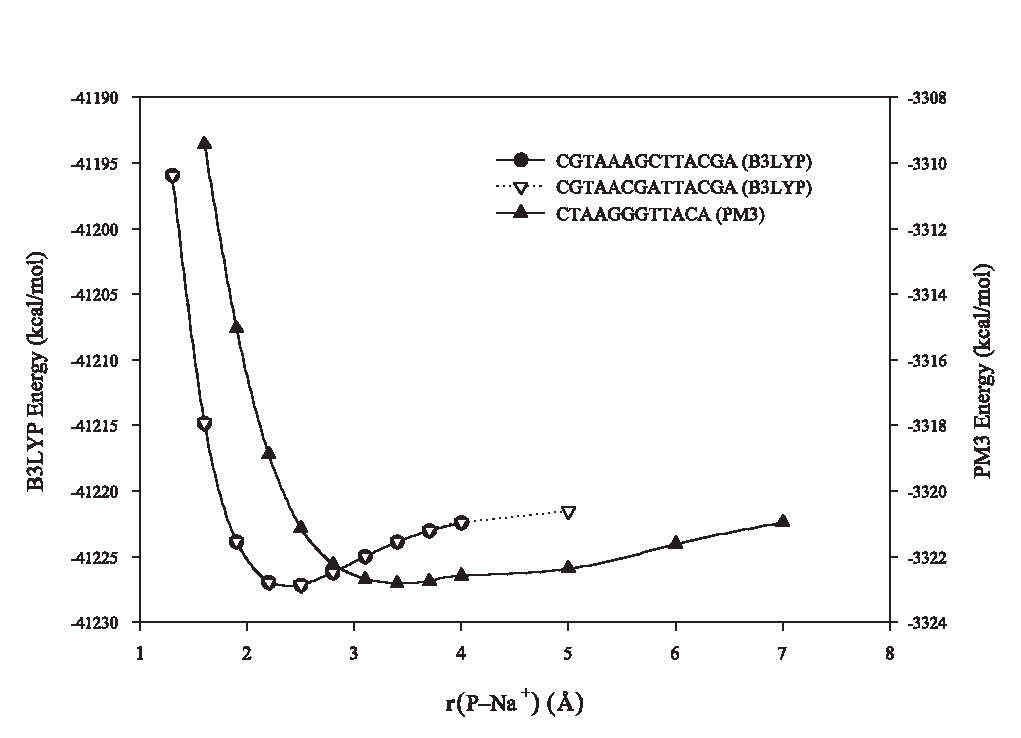
\includegraphics[width=\textwidth]{CationPlacement.eps}
\caption{The cation interaction energies for the two sequences
  calculated at the B3LYP/STO-3G level of theory are essentially
  identical, while the PM3 result shows the lack of dispersion
  treatment inherent in the semiempirical treatment.
  \label{Fig:Cation_Placement}}
\end{figure}

\begin{sidewaystable}
\centering
\begin{tabular}{ccc}
  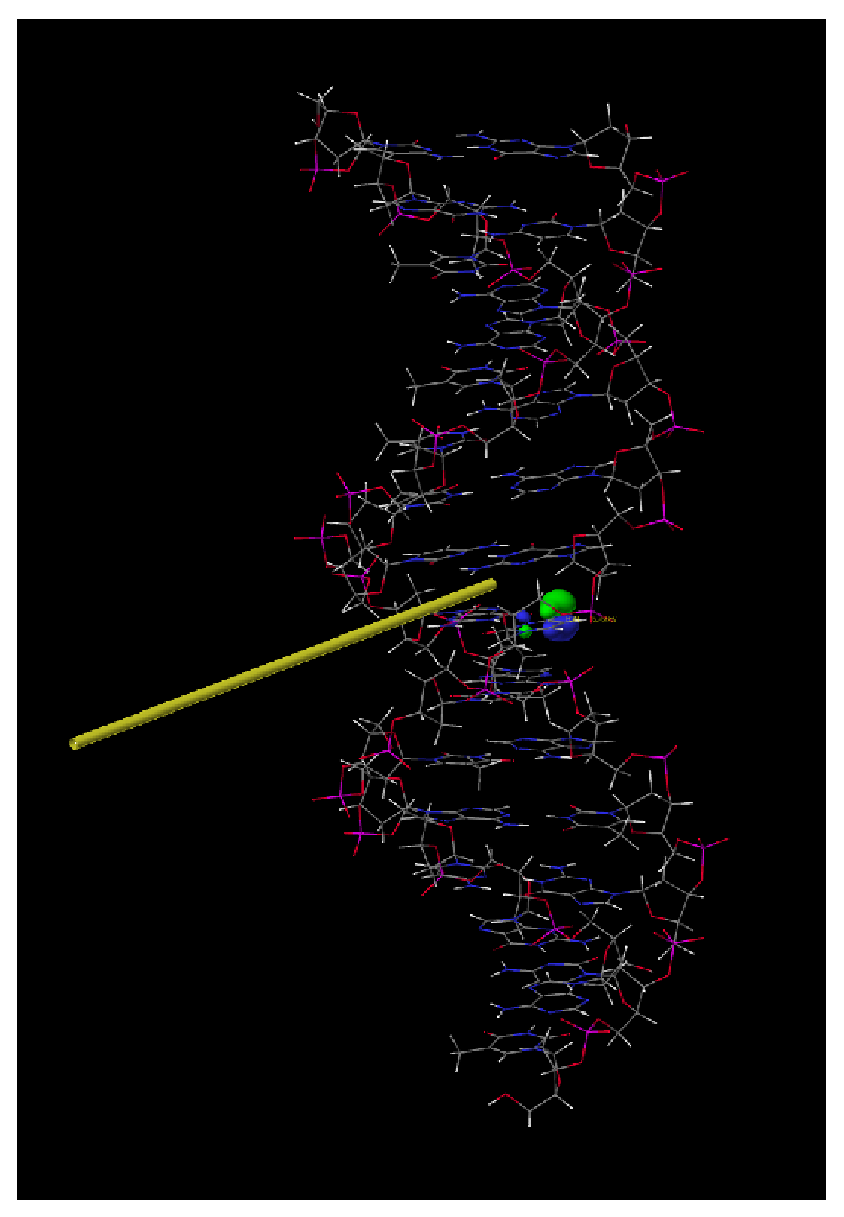
\includegraphics[keepaspectratio,height=3.4in]{YP-15_LocalSCF-PM3-HOMO.v2.eps}
  &
  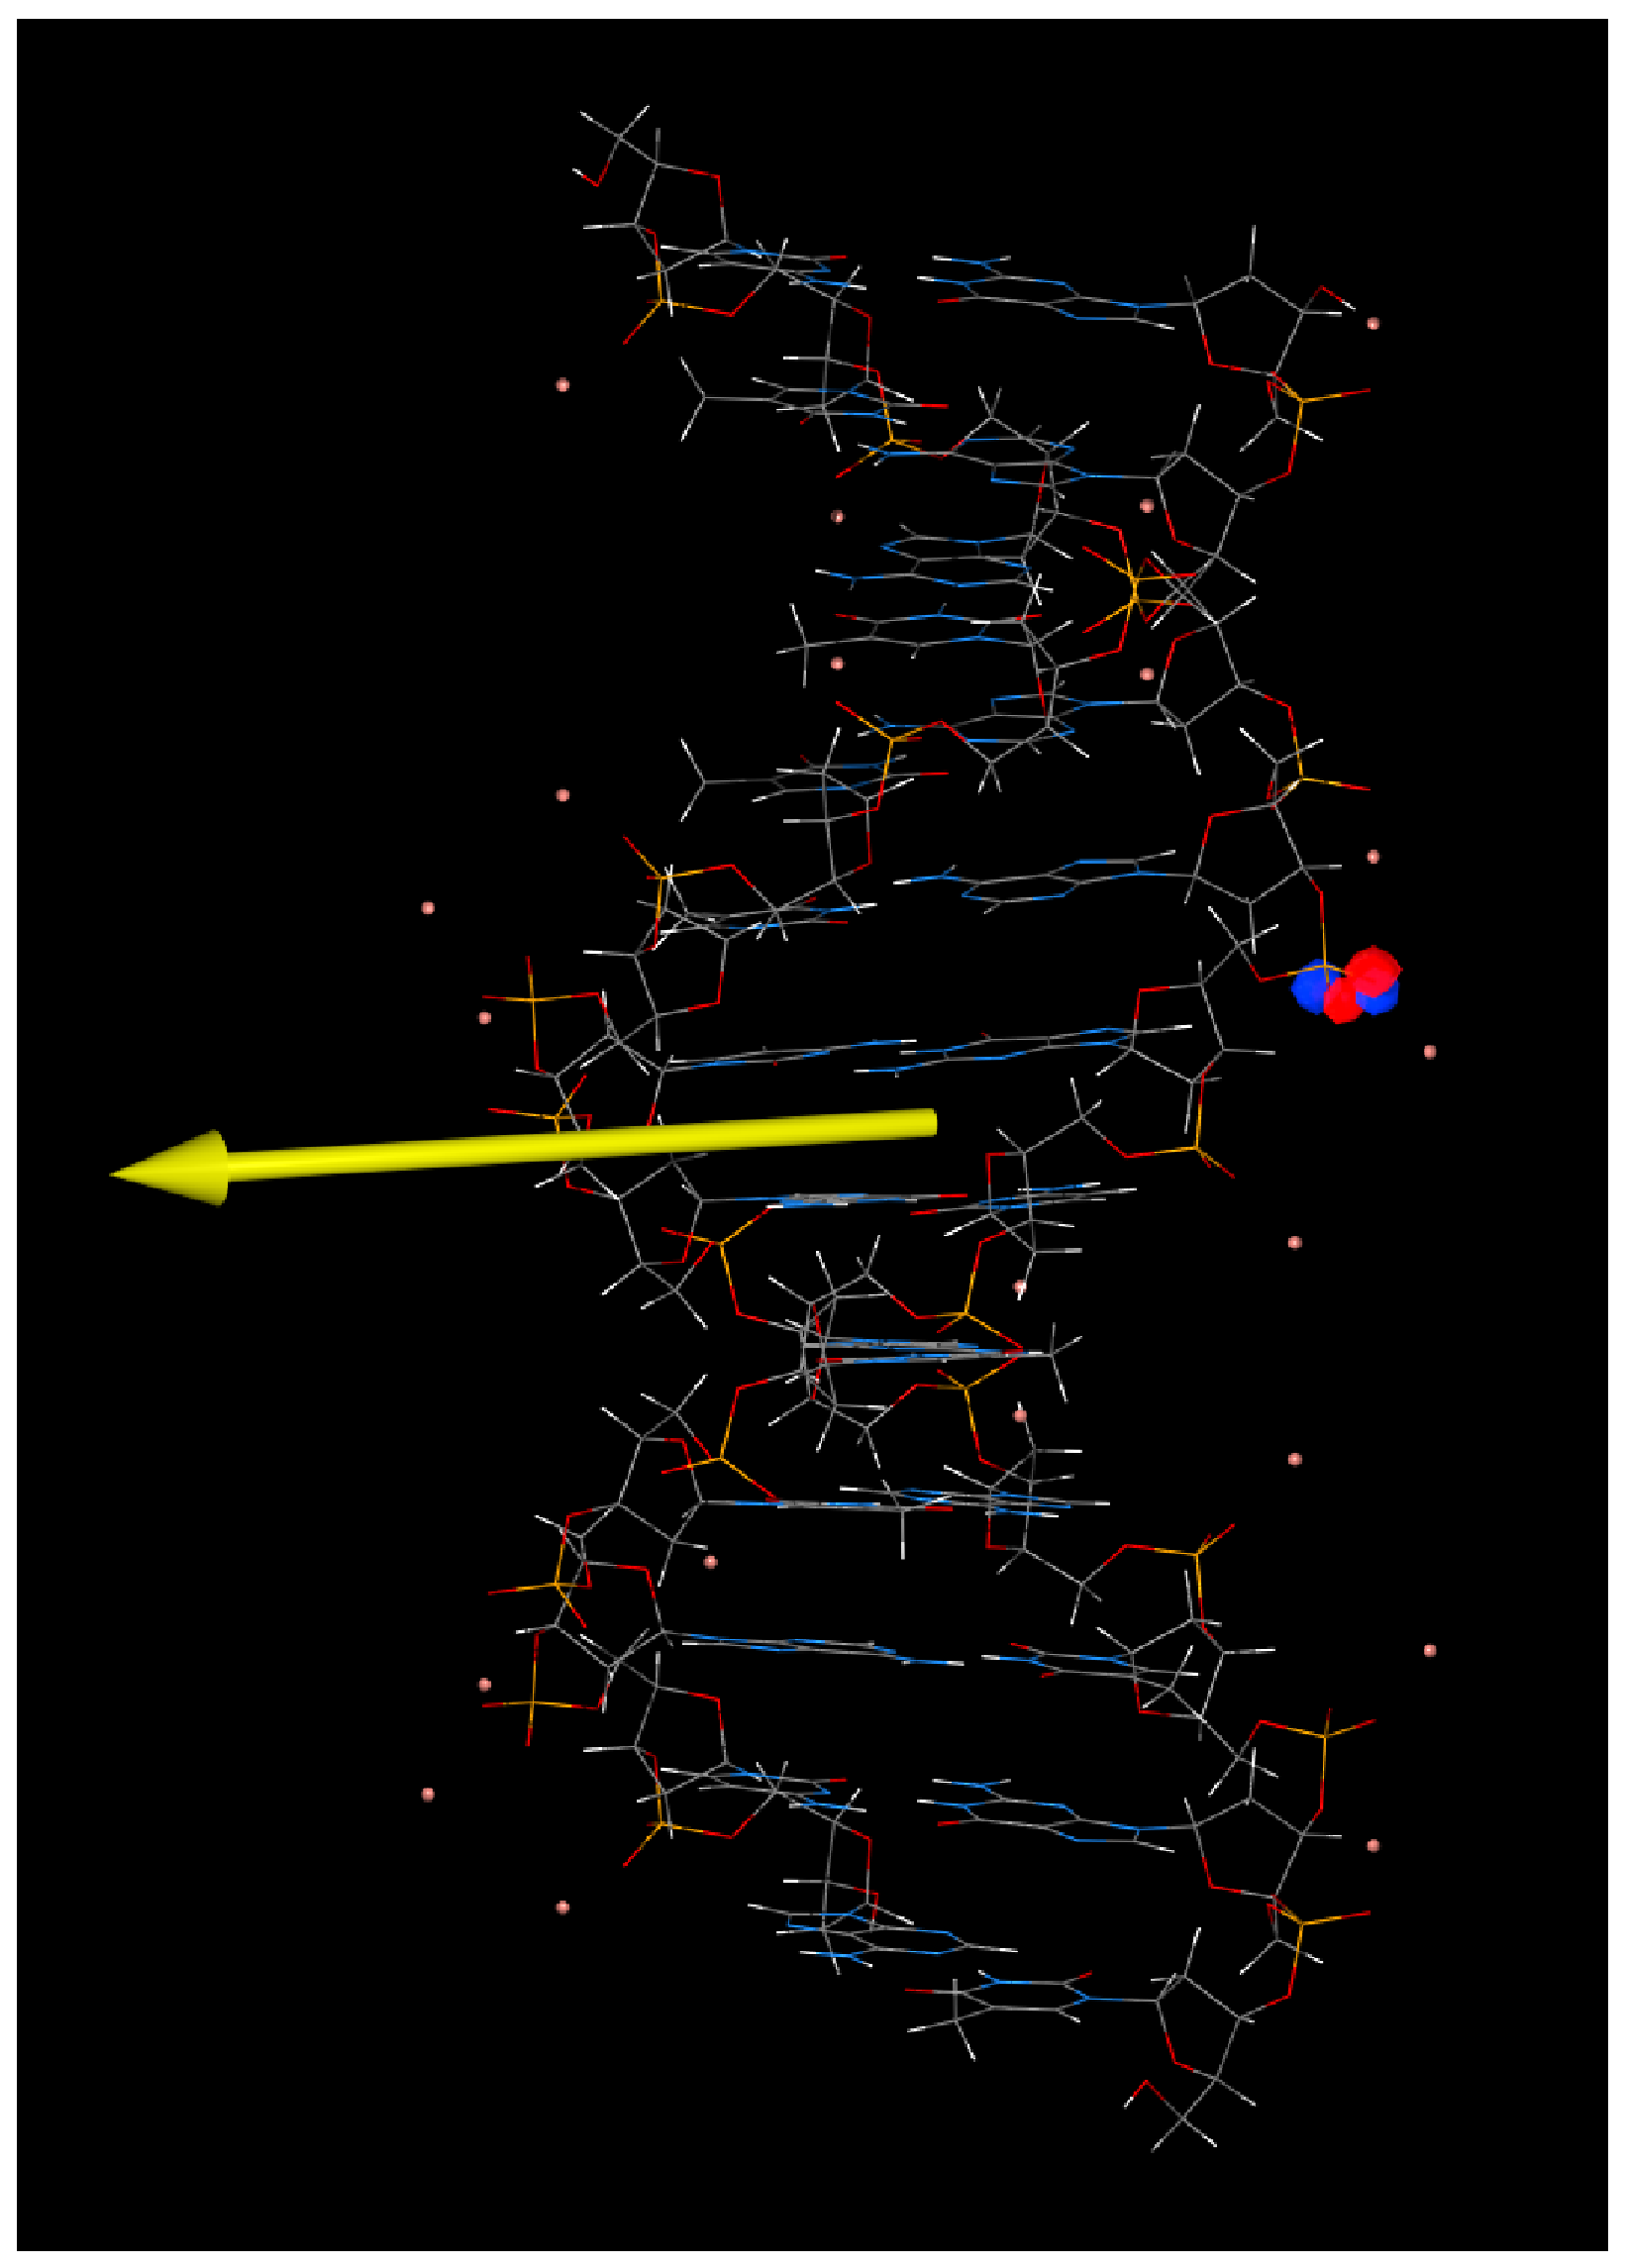
\includegraphics[keepaspectratio,height=3.4in]{YP-15_STO3G-HOMO.v2.eps} &
  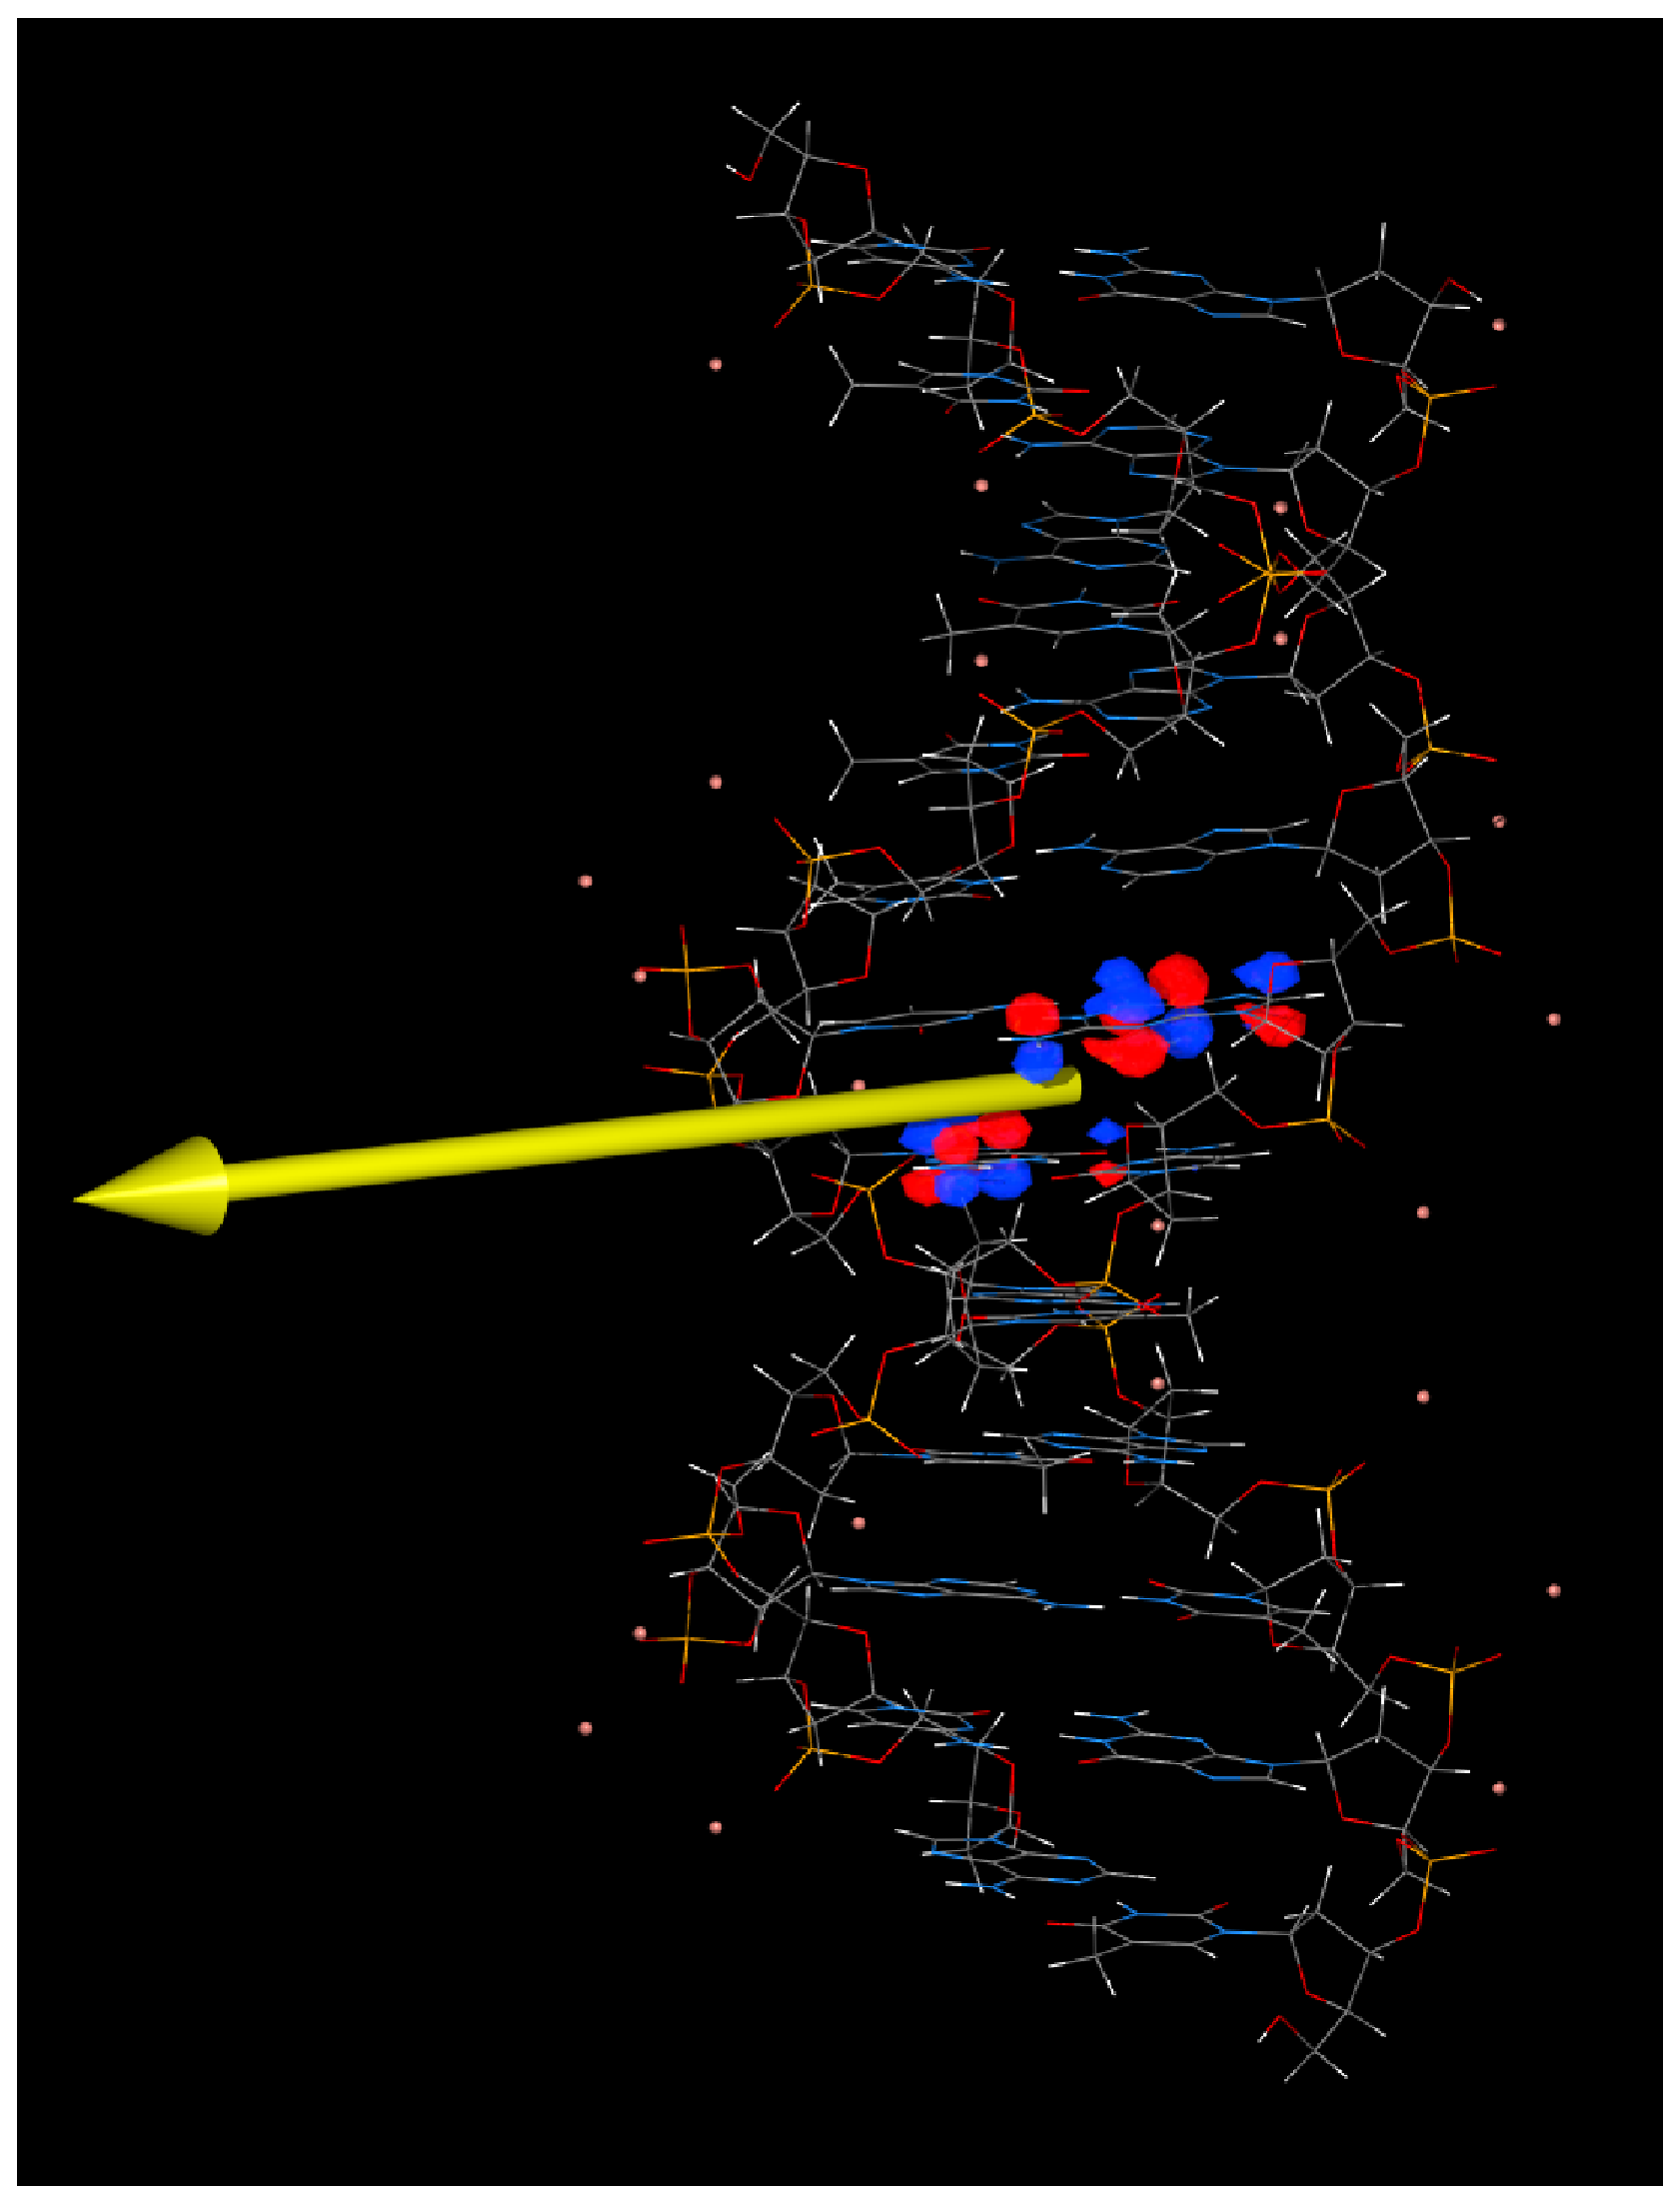
\includegraphics[keepaspectratio,height=3.4in]{YP-15_SBK-HOMO.v2.eps} \\
\end{tabular}
\caption{\label{Fig:LinearScalingOrbitals}}
\end{sidewaystable}


%\begin{figure}[tb]
%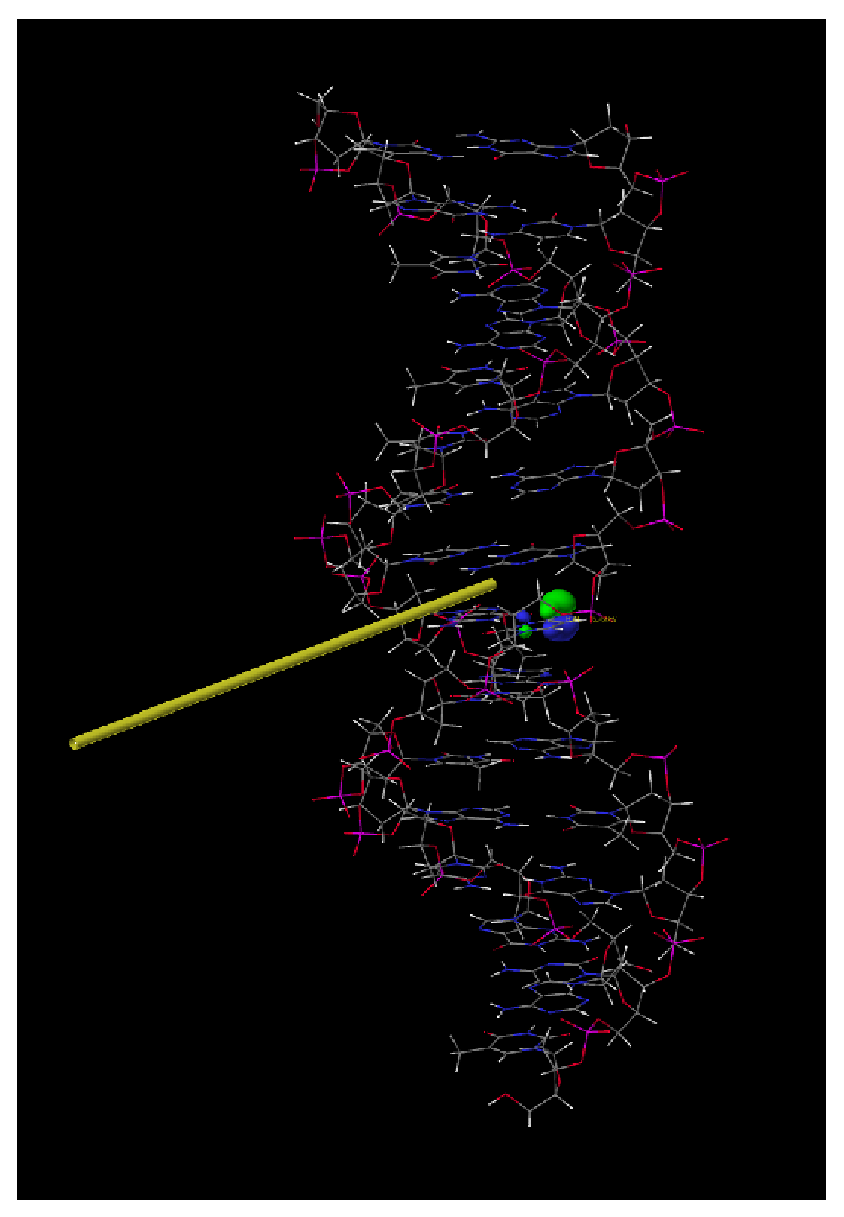
\includegraphics[width=\textwidth]{YP-15_LocalSCF-PM3-HOMO.v2.eps}
%\caption{\label{Fig:YP8_HOMO_alongdipole}}
%\end{figure}

%\begin{figure}[tb]
%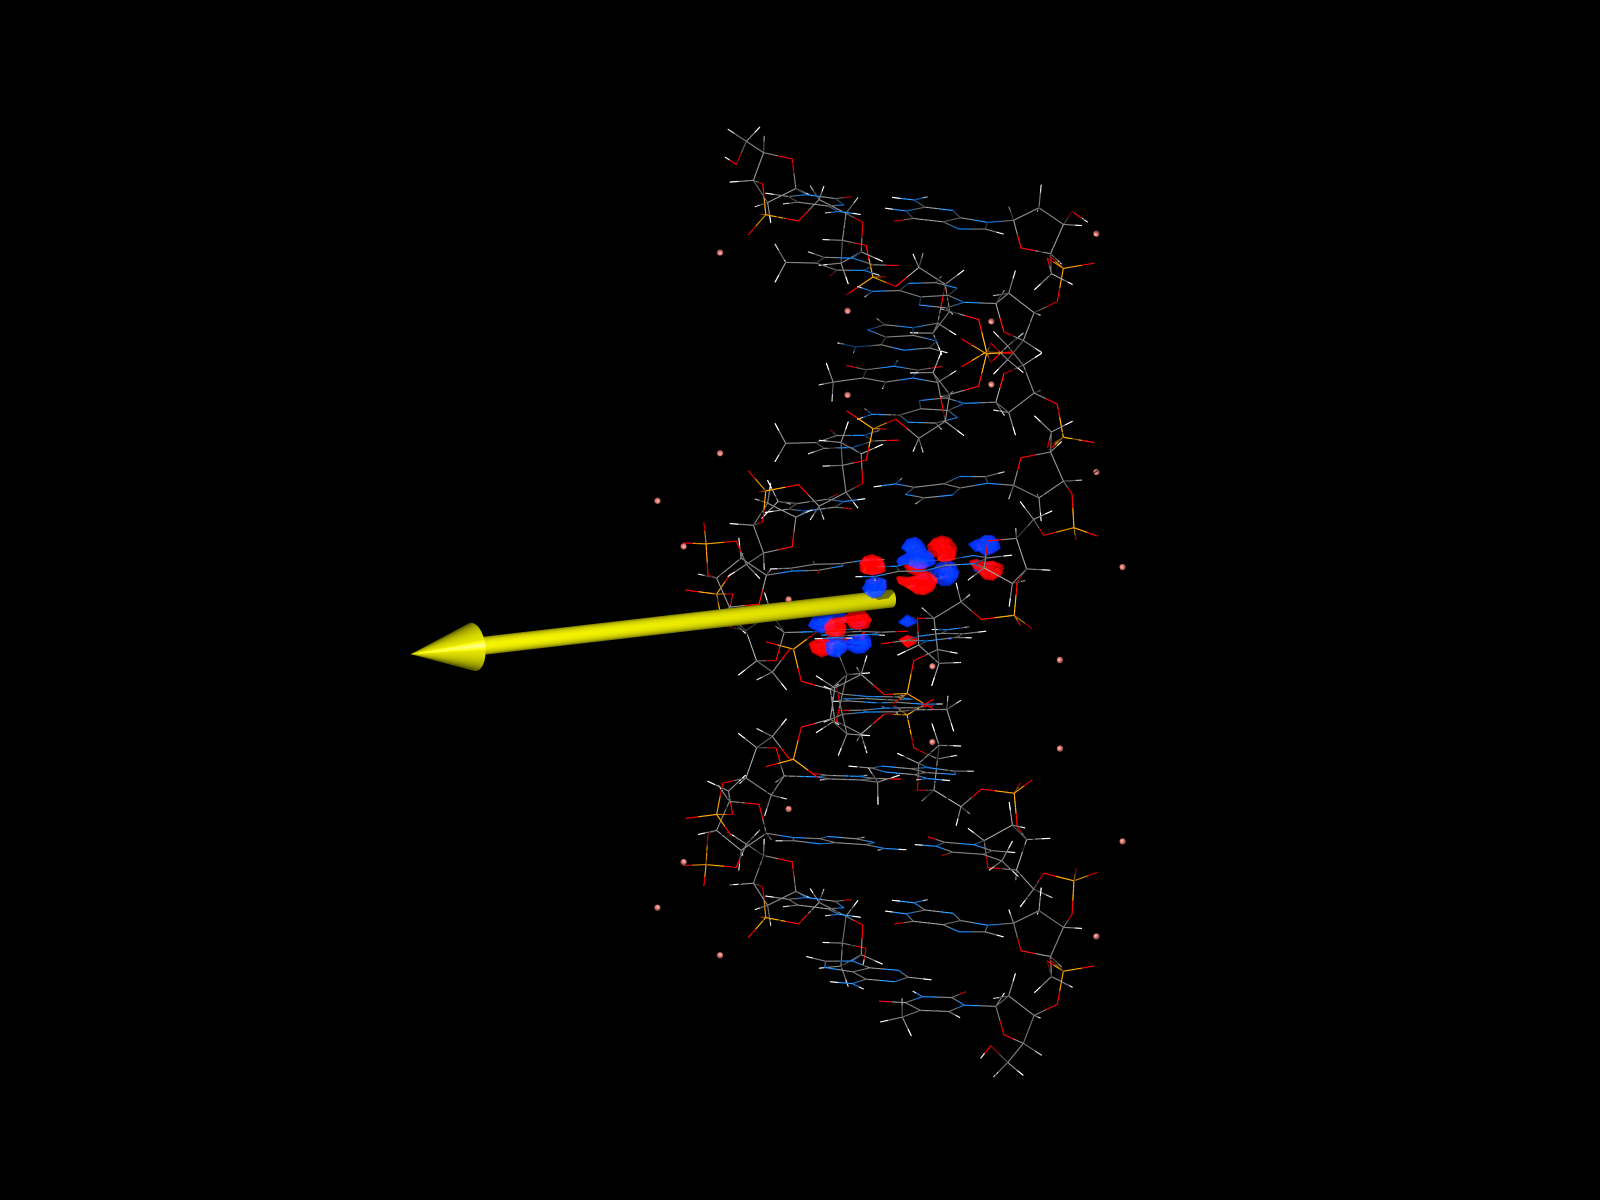
\includegraphics[width=\textwidth]{YP-15_SBK-HOMO.eps}
%\caption{\label{Fig:YP8_HOMO_alongdipole}}
%\end{figure}

%\begin{figure}[tb]
%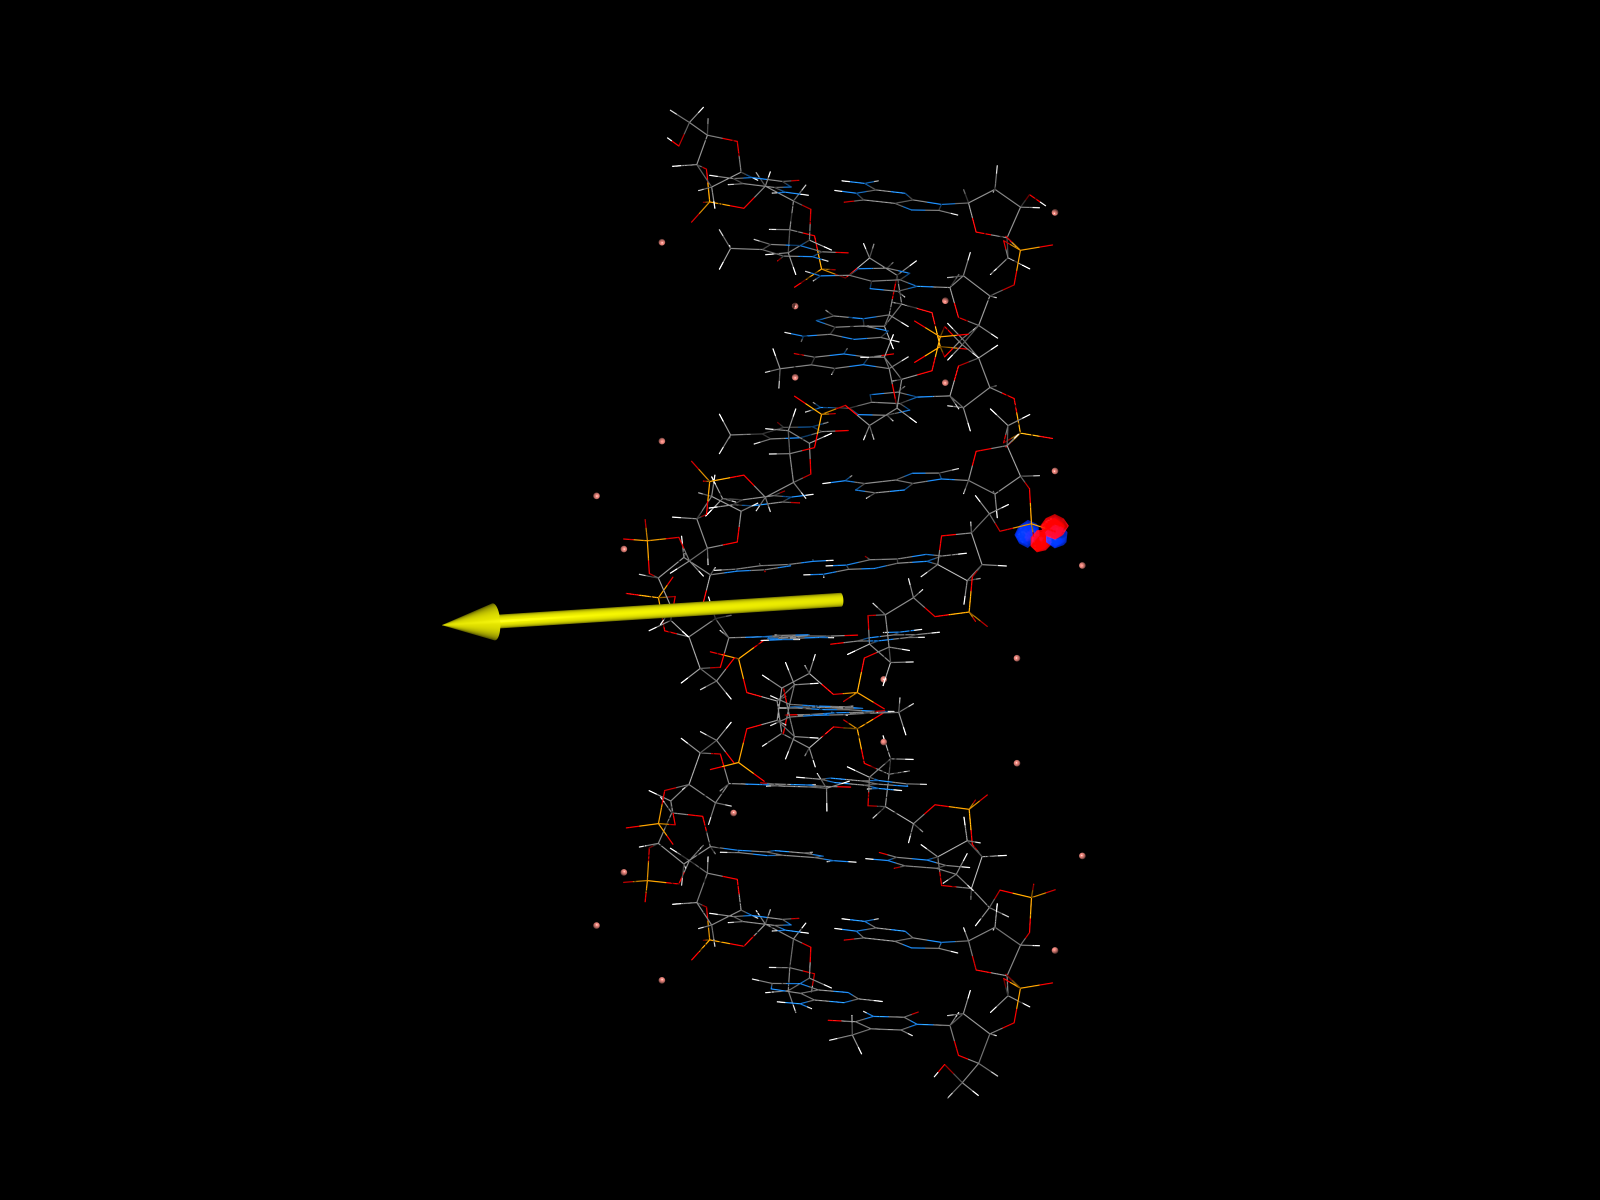
\includegraphics[width=\textwidth]{YP-15_STO3G-HOMO.eps}
%\caption{\label{Fig:YP8_HOMO_alongdipole}}
%\end{figure}

\subsection{Linear Scaling Approximations}
Linear scaling approximations have become a popular method for
treating systems with many hundreds to thousands of atoms quantum
mechanically.  The two most popular implementations are MOZYME method
in Jimmy Stewart's MOPAC2009 package (and previous MOPAC versions from
Fujitsu) and the divide and conquer approach as implemented in DivCon,
which was developed by Kenneth Merz and Lance Westerhoff.
Additionally, the LoaclSCF approach from Victor Anisimov has gained
popularity in recent years.  As the theory behind these approximations
has already been described, we turn our attention to an assessment of
the results obtained from these approaches.




\subsection{Fragment Based Treatments}
[WAITING FOR CALCULATIONS]


\section{Case Study: Ecteinascidin 743}
Having dicussed the considerations necessary for a proper treatment of
large nucleic acid systems, we are now in a position to examine a
particular problem for which electronic structure is of critical
importance.  Namely, the chemical reaction between dsDNA and the
natural product Ecteinascidin 743 (Et-743).  Et-743 is an isolate from
sea squirts and has been prepared by \textit{de novo} synthesis by
Corey and coworkers.  This compound is a DNA methylator, which forms a
bond with the N2 carbon of Guanine bases via minor groove
intercalation.

Pommier\cite{Pommier96} studied the relative kinetics of this reaction
among the sixteen possible sequences in which the central three base
pairs were systematically permuted.  It is somewhat remarkable that
minor permutations in the sequence can lead to drastically different
reaction kinetics.  The explanation for this has been a theory called
\textit{direct readout}.\cite{Hurley98} Under the hypothesis of direct
readout\index{direct readout} an approching chemical enitity is
influenced by changes in electrostatic potential at the exterior of
the double helix caused by variations in the nucleobases at the
interior.  The varying electrostatic interactions allow for favorable
or unfavorable interactions with the minor groove leading to
differential intercalation (and thereby methylation) energetics.

Wether or not subtle sequence variations are sufficient to cause the
requisite charge variation along the phosphate backbone is an
important question that can be addressed using electronic structure
calculations.  As discussed previously, there are several models for
computing atomic charges withing the Hartree-Fock framework.  While
the strengths and shortcomings of each are well known, a qualitative
description is well withing the capabilities of nearly all of the
atomic charge models.  Here we will examine Mulliken charges
calculated using the B3LYP/SBKJC methodology discussed earlier.

For each of the sixteen sequences used in the Pommier experiments, a
B3LYP/SBKJC single-point energy calculation was performed.  Thus, we
have a set of molecular orbitals and a set of atomic charges from
which to work.




\subsection{How Big is Big Enough}
Transcription of information coded in DNA to proteins is a fundamental
process in biological systems.  Codons represent the smallest distinct
unit of information relevant to this process.  Therefore, it is
reasonable to view a codon (three base pairs) as the fundamental unit
that must be accurately described in a treatment of the electronic
structure of DNA.  We wish, then, to answer the following question:
how do we accurately treat the electronic structure of a codon-size
piece of DNA?  Similarly, what is the smallest dsDNA system required
to produce a self-consistent description of the orbitals of a codon?

Developing a practical answer to this question requires an
understanding of what the orbital structure of a three base pair
segment looks like in the context of increasingly extended treatments
with respect to the length of the surrounding sequence.

Accurate calculations of orbital energies are challenging even on
small test systems of dsDNA when counterions are not present.  In
fact, we can see from the results in  Table
\ref{Tab:Trimer_Orbital_Energies} that density functional theory fails
to predict appropriate orbital energies even when given a large basis
set like the polarized Ahlrichs basis set.\ref{basis_pAhlrichs}
Fortunately, removing the core orbitals from the DFT treatment results
in a dramatic improvement of the orbital energies but fails to improve
the difference in the frontier molecular orbitals.  The effective core
potential approach combined with the B3LYP functional seems to give a
fortuitous cancellation of errors and suggests a practical method we
may use to treat larger systems. \marginpar{NOTE: We need to put the
  orbital energies obtained \textbf{with} the counterions into this table!}.


\begin{sidewaystable}
  \begin{tabular}{lrrrrrrrr}
                    & B3LYP/ & B3LYP/     & B3LYP/  & HF/     & MP2/    & B3LYP/  & B3LYP/     & B3LYP/  \\
  Orbital           & 3-21G  & 6-31G($d$) & cc-pVDZ & cc-pVDZ & cc-pVDZ & cc-pVTZ & p-Ahlrichs & SBKJC   \\
  \hline\\[0.5ex]
  $\mathrm{LUMO}+5$ & 0.2144 & 0.2087     & 0.2083  &  0.3550 &  0.3550 &  0.1981 & 0.2032     &  0.1937 \\
  $\mathrm{LUMO}+4$ & 0.2123 & 0.2042     & 0.2031  &  0.3478 &  0.3478 &  0.1894 & 0.1988     &  0.1884 \\
  $\mathrm{LUMO}+3$ & 0.2021 & 0.1917     & 0.1903  &  0.3319 &  0.3319 &  0.1780 & 0.1855     &  0.1774 \\
  $\mathrm{LUMO}+2$ & 0.1898 & 0.1849     & 0.1839  &  0.3273 &  0.3273 &  0.1730 & 0.1793     &  0.1712 \\
  $\mathrm{LUMO}+1$ & 0.1874 & 0.1809     & 0.1807  &  0.3176 &  0.3176 &  0.1691 & 0.1752     &  0.1652 \\
  $\mathrm{LUMO}$   & 0.1857 & 0.1776     & 0.1766  &  0.3163 &  0.3162 &  0.1655 & 0.1716     &  0.1641 \\
  $\mathrm{HOMO}$   & 0.0471 & 0.0407     & 0.0415  & -0.0465 & -0.0465 &  0.0289 & 0.0357     &  0.0222 \\
  $\mathrm{HOMO}-1$ & 0.0348 & 0.0126     & 0.0154  & -0.0763 & -0.0763 &  0.0019 & 0.0115     & -0.0038 \\
  $\mathrm{HOMO}-2$ & 0.0318 & 0.0123     & 0.0128  & -0.0925 & -0.0925 & -0.0052 & 0.0075     & -0.0139 \\
  $\mathrm{HOMO}-3$ & 0.0247 & 0.0057     & 0.0077  & -0.1074 & -0.1074 & -0.0100 & 0.0033     & -0.0166 \\
  $\mathrm{HOMO}-4$ & 0.0243 & 0.0040     & 0.0062  & -0.1182 & -0.1182 & -0.0111 & 0.0020     & -0.0177 \\
  $\mathrm{HOMO}-5$ & 0.0223 & 0.0027     & 0.0057  & -0.1240 & -0.1240 & -0.0124 & 0.0015     & -0.0191 \\
  \hline\\[0.5ex]
  $\varepsilon_\mathrm{LUMO} - \varepsilon_\mathrm{HOMO}$ &
                      0.1386 & 0.1369     & 0.1351  & 0.3628  & 0.3627  &  0.1366 & 0.1359     &  0.1419 \\
  \hline\\[0.5ex]
  \end{tabular}
  \caption{Comparison of the calculated orbital energies for the
  d(AGC) system using various basis sets.  It is interesting to note
  that the density functional theory calculations consistently
  underestimate the HOMO--LUMO gap and that only the Hartree--Fock
  methods predict that all occupied states are bound.\label{Tab:Trimer_Orbital_Energies}}
\end{sidewaystable}


\subsection{It's all about the orbitals}


\begin{table}
\begin{tabular}{lllllll}
 & \multicolumn{2}{c}{CTAA\underline{TGT}TTACA} & 
   \multicolumn{2}{c}{CTAA\underline{TGG}TTACA} &
   \multicolumn{2}{c}{CTAA\underline{AGC}TTACA} \\
 & P & Na & P & Na & P & Na \\
\hline\\[0.5ex]
1         & 0.4510 & 0.8589 & 0.4510 & 0.8591 & 0.4544 & 0.8589 \\
2         & 0.4507 & 0.8567 & 0.4507 & 0.8570 & 0.4517 & 0.8550 \\
3         & 0.4507 & 0.8556 & 0.4508 & 0.8561 & 0.4357 & 0.8562 \\
4         & 0.4540 & 0.8559 & 0.4538 & 0.8566 & 0.4510 & 0.8542 \\
5         & 0.4522 & 0.8561 & 0.4489 & 0.8544 & 0.4485 & 0.8520 \\
6         & 0.4479 & 0.8528 & 0.4467 & 0.8518 & 0.4468 & 0.8557 \\
7         & 0.4503 & 0.8529 & 0.4523 & 0.8518 & 0.4512 & 0.8564 \\
8         & 0.4504 & 0.8530 & 0.4507 & 0.8523 & 0.4518 & 0.8566 \\
9         & 0.4498 & 0.8550 & 0.4498 & 0.8544 & 0.4549 & 0.8555 \\
10        & 0.4552 & 0.8574 & 0.4551 & 0.8569 & 0.4538 & 0.8547 \\
11        & 0.4572 & 0.8611 & 0.4572 & 0.8609 & 0.4483 & 0.8568 \\
\hline\\[0.5ex]
Average   & 0.4518 & 0.8559 & 0.4515 & 0.8556 & 0.4515 & 0.8556 \\
Std. Dev. & 0.0027 & 0.0026 & 0.0029 & 0.0030 & 0.0027 & 0.0017 \\
Range     & 0.0093 & 0.0083 & 0.0105 & 0.0091 & 0.0080 & 0.0069 \\
\end{tabular}
\caption{Comparison of the charge variation along the backbone of three
         distinct dsDNA sequences.  The central three bases correspond
         to sequences with poor, moderate, and good alkylation as observed
         in the experiments of Pommier.  Interestingly, the sequence with
         the most efficient alkylation shows the lowest charge variation
         among the backbone phosphorous atoms and the sodium counterions.
         \label{Tab:Phosphate_Charges}}
\end{table}

In order to examine the question about charge variation along the DNA
backbone, we calculated the Mulliken charges for
ds(CTAA\textbf{XXX}TTACA), where \textbf{XXX} = TGT, TGG, and AGC,
using B3LYP/SBKJC.  Results for the P atoms and the Na counterions are
reported in Table \ref{Tab:Phosphate_Charges}.  \marginpar{Q: Should
we report the average charge on the exocyclic O atoms as well?}  We
have chosen to examine the charge density on the P atoms for two
reasons.  Firstly, they are directly bonded to the atoms that should
show the greatest charge variation along the backbone.  Namely the
exocyclic oxygen atoms, which are highly polarizable because of the
$d$-bonding present in phosphates.  If there is charge variation along
the backbone these oxygens should be perturbed by virtue of their
polarizable electron density.  Secondly, if the bases interior to the
double helix are responsible for creating charge variation along the
backbone, they will have to do so (at least in part) through an
inductive effect.  Any perturbation of the backbone charges must
effect the P atoms either by perturbing the charge in the ribose rings
or through direct inductive effects exhibited through bond
polarization.  Examining the charge on the Na cations is done
primarily as a reference.  These cations are closed-shell species and
do not interact with the orbitals of the dsDNA directly, an assertion
that is easily verified by examining which orbitals contain non-zero
AO coefficients from the Na orbitals.  There should be no appreciable
charge variation for these cations and their interaction with any
electron in the nucleic acid system will be purely electrostatic.

These calculations show remarkably little charge variation among the P
atoms, with varations measured in the hundreths to thousandsth of a
charge unit.  Comparing the charge variation to that of the reference
cations suggests that there is actually no appreciable charge
variation along the phosphate backbone.  In order for the hypothesis
of direct readout to work, charge variations of at most $0.105\,e$
would have to influence the electrostatic interactions between the
intercalating ligand and the dsDNA substrate.  This seems highly
unlikely given the solvent dielectric constant screening the backbone
charge from any approaching ligand.  In the absence of an appreciable
charge variation along the backbone to explain the sequence
specificity of Et-743 as an intercalating species, we turn to
electronic structure theory for a possible explanation.









\begin{figure}[tb]
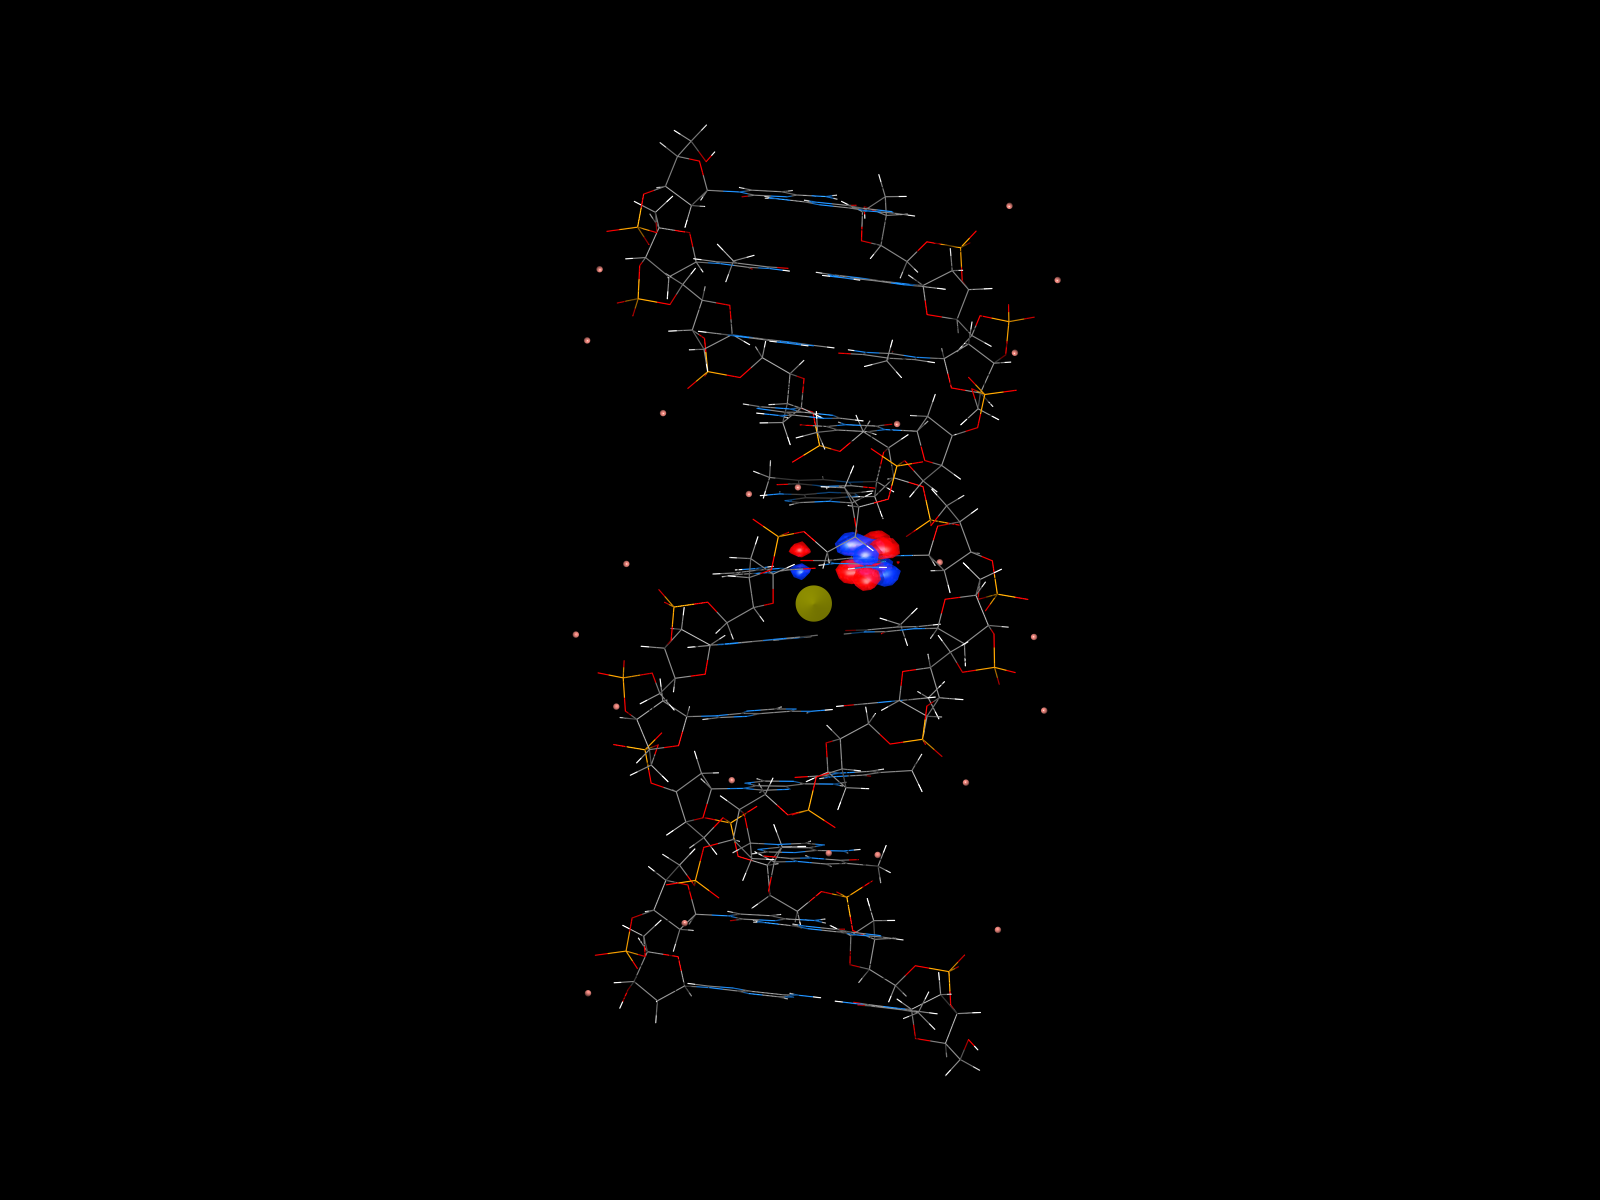
\includegraphics[width=\textwidth]{YP-08_SBK-HOMO.downDipole.eps}
\caption{\label{Fig:YP8_HOMO_alongdipole}}
\end{figure}

\begin{figure}[tb]
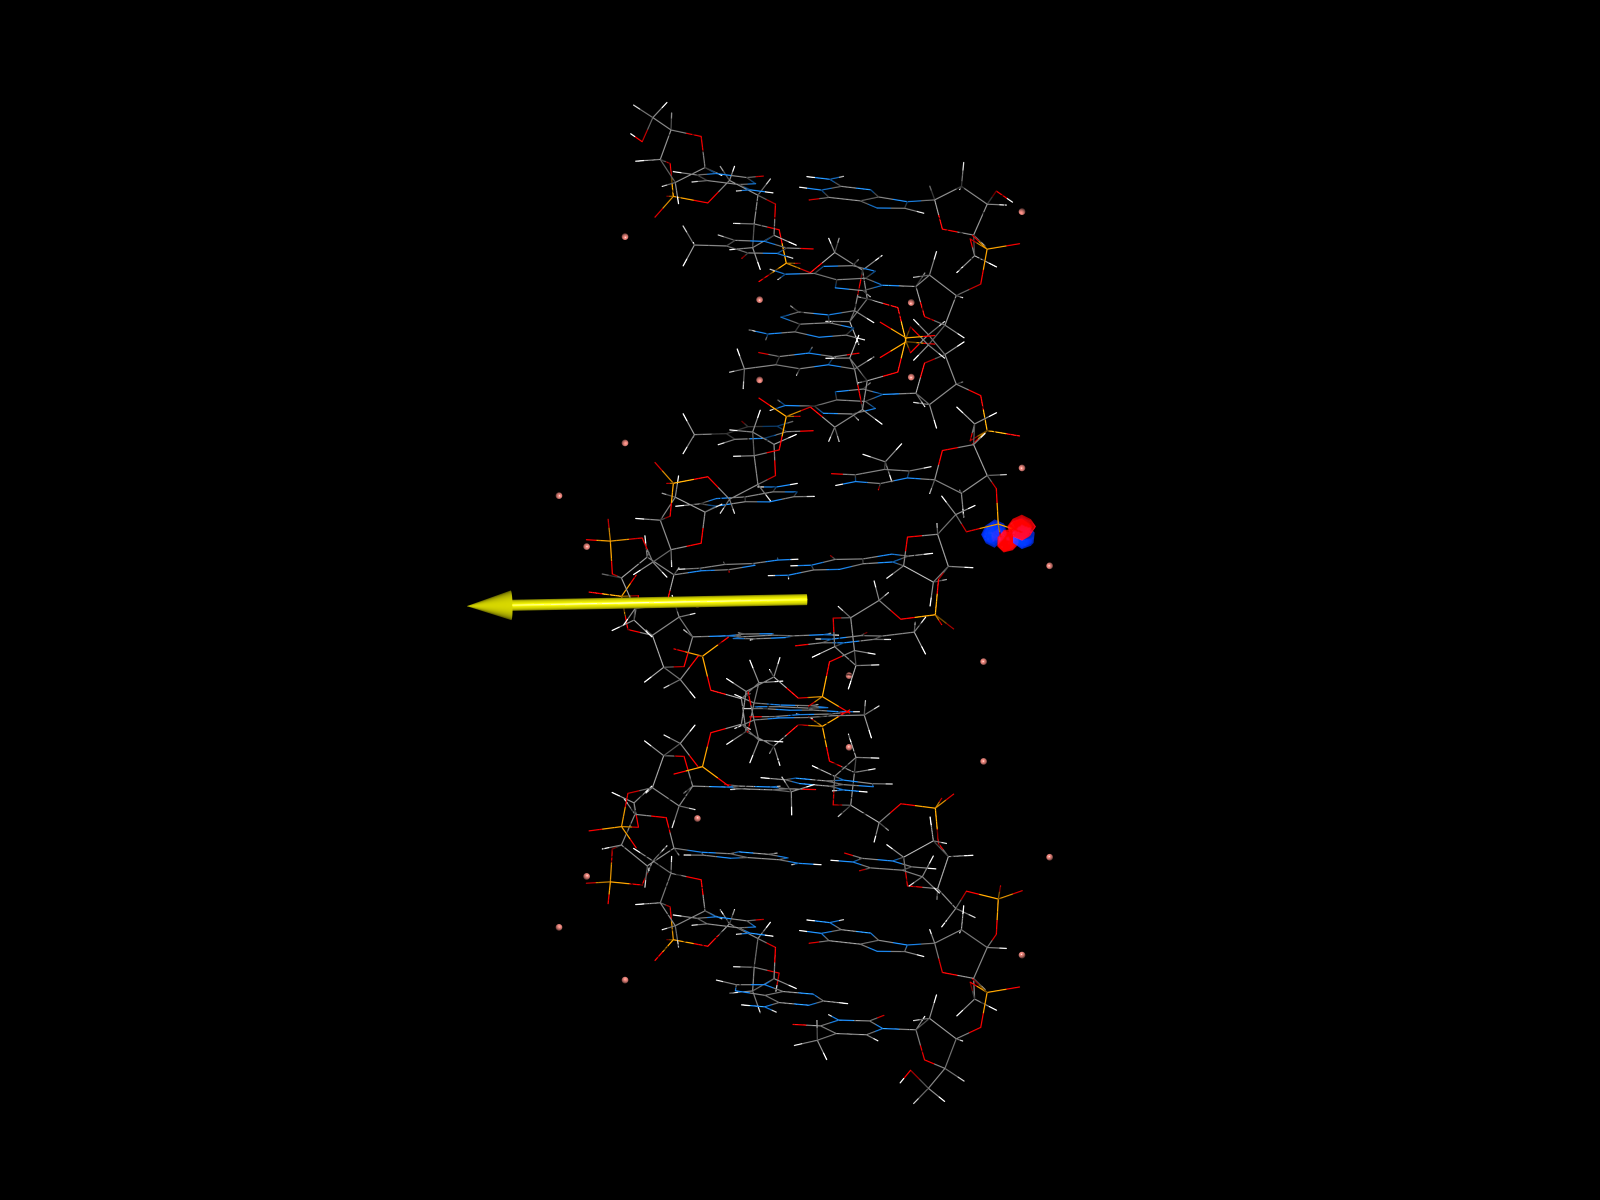
\includegraphics[width=\textwidth]{YP-08_STO3G-HOMO.eps}
\caption{\label{Fig:YP8_HOMO_alongdipole}}
\end{figure}



\begin{figure}[tb]
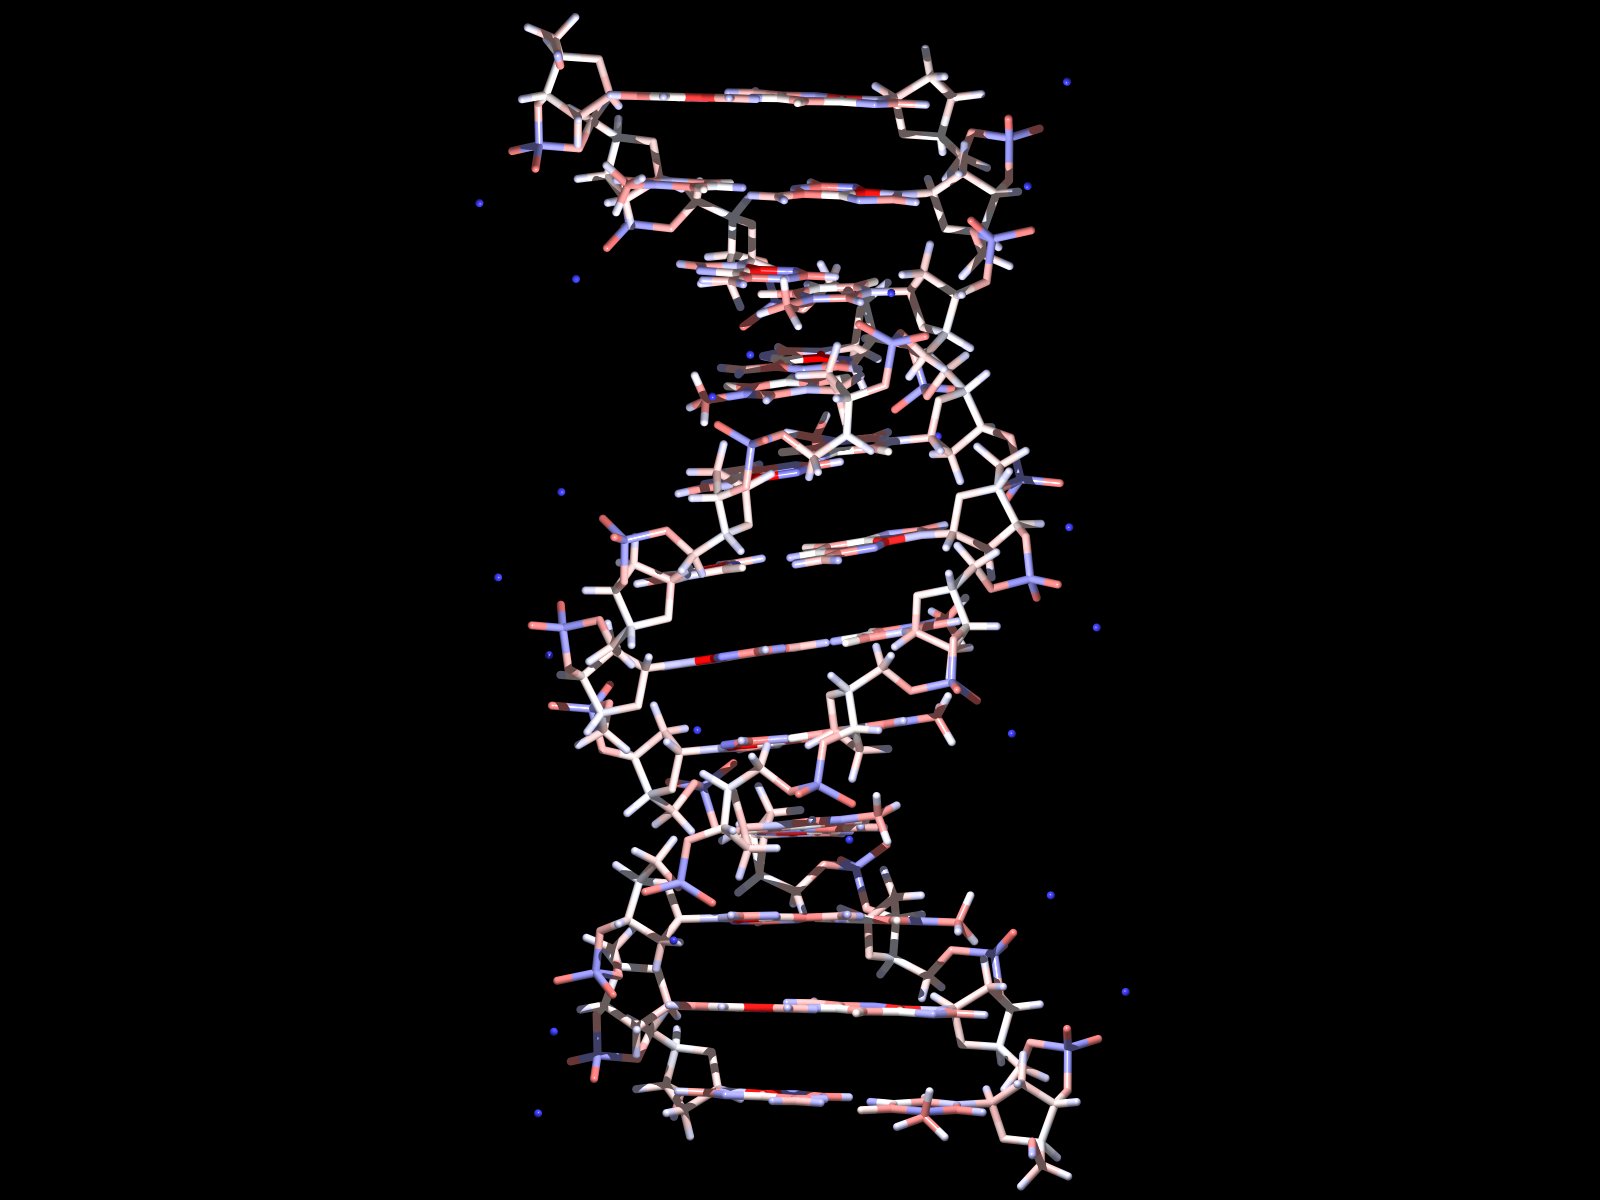
\includegraphics[width=\textwidth]{YP-08-SBK-Charge.eps}
\caption{\label{Fig:YP8_HOMO_alongdipole}}
\end{figure}

\begin{figure}[tb]
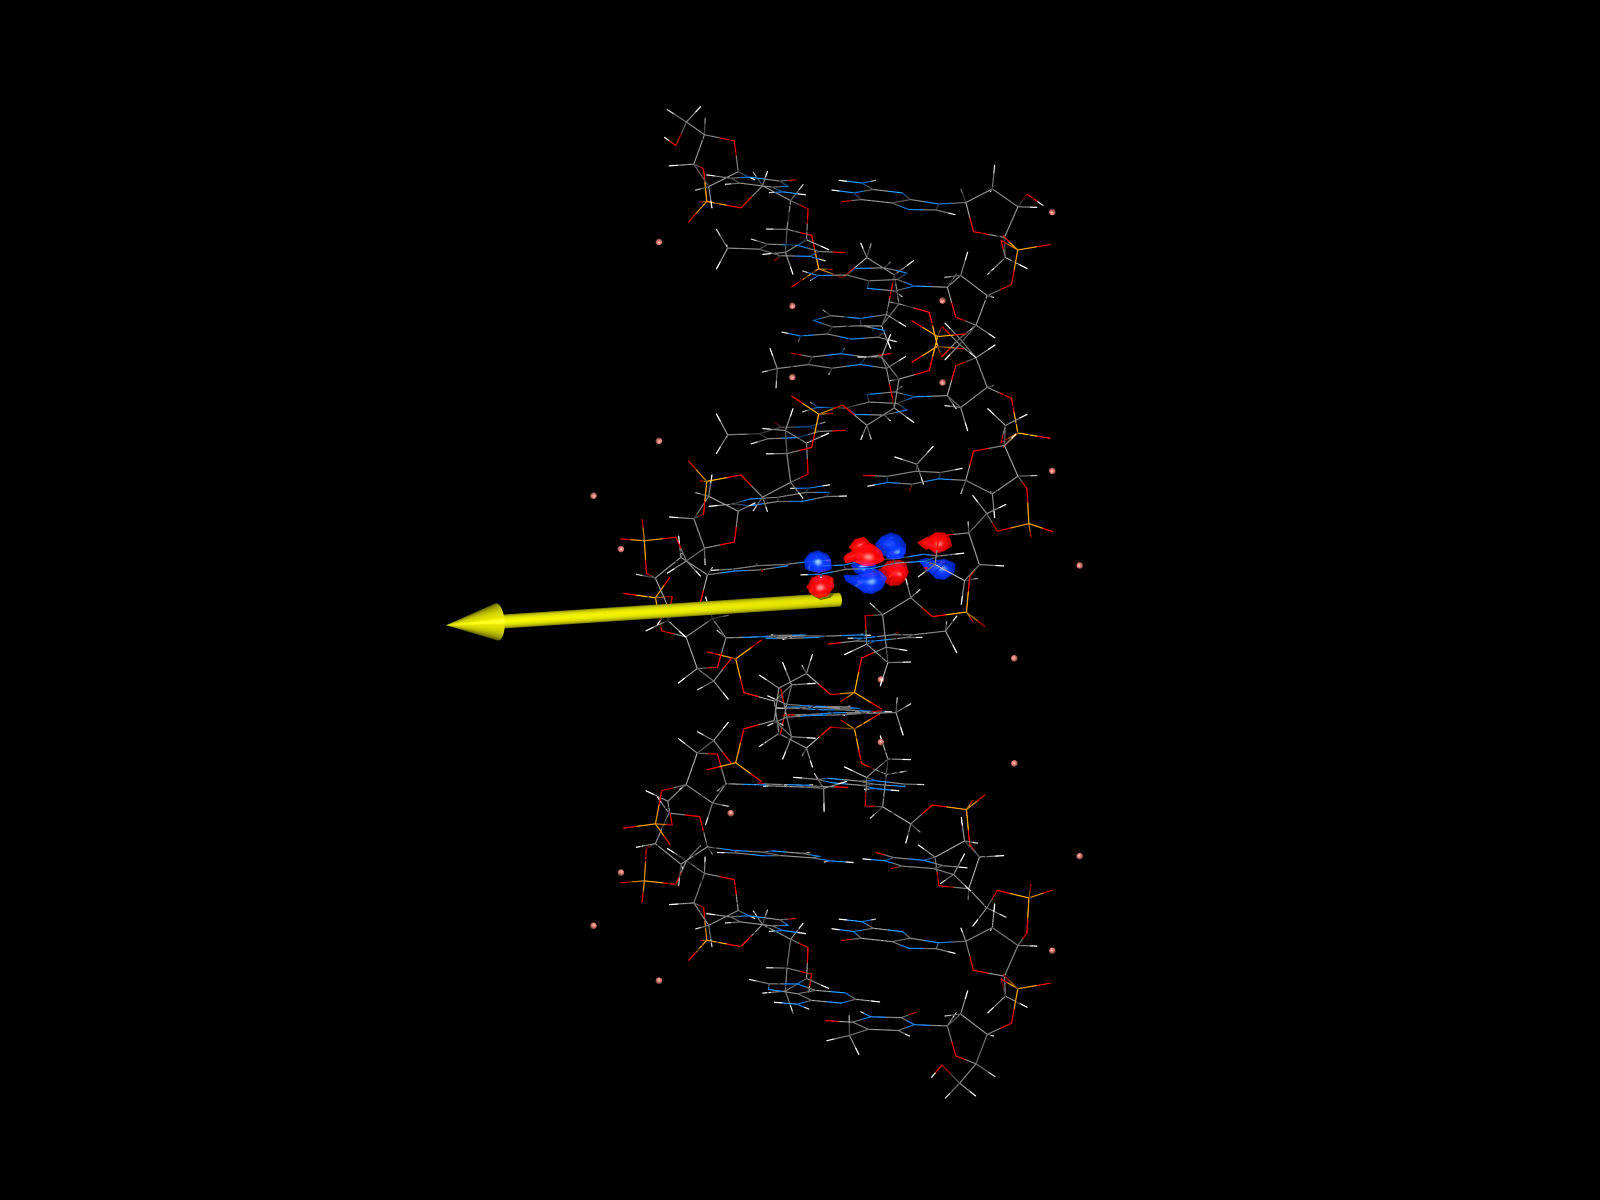
\includegraphics[width=\textwidth]{YP-08_SBK-HOMO.eps}
\caption{\label{Fig:YP8_HOMO_alongdipole}}
\end{figure}


\begin{figure}[tb]
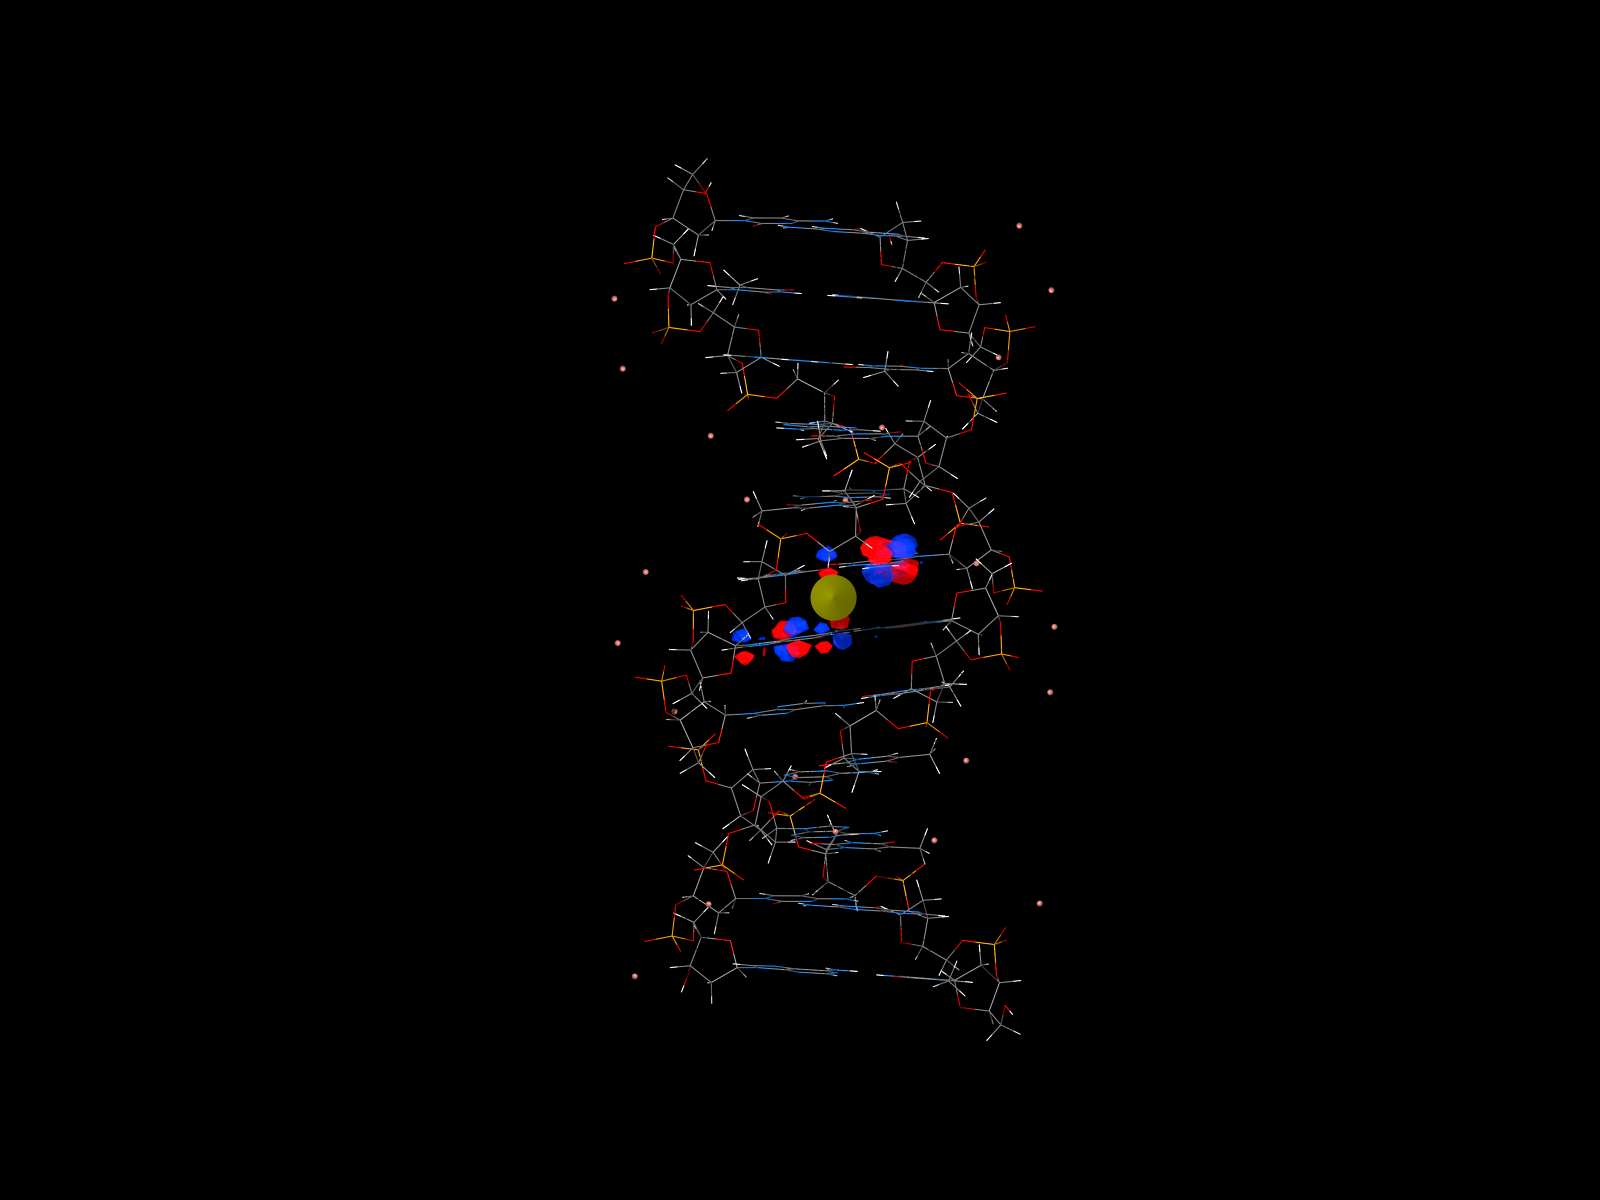
\includegraphics[width=\textwidth]{YP-15_SBK-HOMO.downDipole.eps}
\caption{\label{Fig:YP8_HOMO_alongdipole}}
\end{figure}

